
%%%%%%%%%%%%%%% 集合 %%%%%%%%%%%%%

\chapter{集合}

集合的理论是所有数学理论的基础系统。在这一章中我们将简单地介绍集合的一些基本理论。我们采用较自然及直觉的方式介绍集合论，而不涉及抽象的公设结构。

\section{基本定义}

首先我们介绍有关集合的基本定义，并了解集合之间的关系。

集合和元素是数学最基本的名词，严格说起来它是无法定义清楚的。这里我们就不去定义集合，而采用较直观的说法。所谓一个\textbf{集合（set）}\index{集合（set）}就是一些事物收集起来的结果，而组成这个集合的事物，我们称为此集合的\textbf{元素（element）}。\index{元素（element）}通常我们会用英文大写来表示一个集合，例如 $A, B, S$ 等，而用小写字母来表示集合里的元素。不过有些数学常用的集合大家都习惯用特定的符号表示。例如：$\mathbb{N}$ 表示所有自然数所成的集合，$\mathbb{Z}$ 为整数所成的集合，$\mathbb{Q}$ 表示有理数所成的集合，而所有实数所成的集合我们用 $\mathbb{R}$ 来表示。若 $x$ 为集合 $S$ 里的一个元素，我们就用 $x \in S$ 来表示，称之为 $x$ \textbf{属于（belong to）}$S$。\index{属于（belong to）}若 $x$ 不在 $S$ 中，我们就用 $x \notin S$ 来表示。

在数学上，我们希望一个集合是要明确地知道哪些是它的元素、哪些不是它的元素。也就是说给定一集合 $S$，对于任意的 $x$，我们必须明确知道 $x \in S$ 是对的还是错的。一般来说，一个集合若仅有有限多个元素，我们便可以一一将它们列举出来。例如 $S = \{1, 2, 3\}$ 表示的就是有 3 个元素的集合，其元素为 $1, 2$ 和 $3$。这里 $S$ 是一个集合，例如我们知道 $1 \in S$，而 $4 \notin S$。有时一个集合我们无法一一列举出它的元素，此时我们便用所谓\textbf{集合建构式符号（set-builder notation）}\index{集合建构式符号（set-builder notation）} 来表示其元素。它的表示法通常为 $\{x : P(x)\}$ 这样的形式，其中冒号左边的 $x$ 表示我们要用 $x$ 来表示此集合的元素，而冒号右边的 $P(x)$ 指的是这个集合里的元素 $x$ 需满足 $P(x)$。也就是说 $\{x : P(x)\}$ 这个集合便是收集所有满足 $P(x)$ 的 $x$ 所成的集合。

在探讨集合相关性质之前，首先我们必须定义何谓集合的相等，以及集合间的包含关系。

\begin{definition}
设 $A, B$ 为集合。如果 $B$ 中的元素皆为 $A$ 的元素，我们称 $B$ 为 $A$ 的{\bf 子集（subset）}，\index{子集（subset）}也称 $B$ {\bf 包含于（is contained in）}\index{包含于（is contained in）} $A$，记为 $B \subseteq A$。若 $B \subseteq A$ 且 $A \subseteq B$，则称 $A, B$ 为{\bf 相等（equal）}，记为 $A = B$。另外若 $B \subseteq A$ 但 $B \neq A$，则称 $B$ 为 $A$ 的{\bf 真子集（proper subset）}，\index{真子集（proper subset）}记为 $B \subset A$。
\end{definition}

注意子集和真子集的符号 “$\subseteq$” 和 “$\subset$”，许多参考书籍的符号并不一致，请在阅读时注意\footnote{有的书将$\subset$记为$\subsetneq$。——译者注}。

依定义若要证明 $B \subseteq A$，我们必须说明任意 $B$ 中的元素 $x$，皆会是 $A$ 的元素，所以用数学的表示法就是要证明 “$x \in B \Rightarrow x \in A$”。而要证明 $A = B$ 的话就是等同于证明 “$x \in B \Leftrightarrow x \in A$”。从这里得知，两集合的包含关系以及相等，只与元素是否属于该集合有关，和集合的表示法无关。例如以下的例子：

\begin{example}
令 $A = \{1, 2, 2\}$, $B = \{1, 2, 3\}$, $C = \{3, 3, 1, 2\}$, $D = \{n \in \mathbb{N} : 1 \leq n \leq 3\}$, $E = \{2, 4\}$\footnote{在花括号内列举出来元素$x$表示$x$属于这个集合，数学学界一般允许列举法中存在重复元素，注意这点与大陆高中教材不一样——译者注}。

由于 $A$ 仅有 $1, 2$ 两个元素，而 $1 \in B$ 且 $2 \in B$，故知 $A \subseteq B$。又 $3 \in B$ 但 $3 \notin A$，知 $B$ 不包含于 $A$，故得 $A \subset B$。同理我们知 $B = C$。

现若 $x \in B$，则知 $x \in \mathbb{N}$ 且 $1 \leq x \leq 3$，故得 $x \in D$。得证 $B \subseteq D$。另一方面，若 $x \in D$ 表示 $x \in \mathbb{N}$ 且 $1 \leq x \leq 3$，所以 $x = 1, 2, 3$ 皆在 $B$ 中，得证 $D \subseteq B$，由此知 $B = D$。

最后因 $1 \in B$ 但 $1 \notin E$，我们知 $B$ 不是 $E$ 的子集。同样地，因 $4 \in E$ 但 $4 \notin B$，我们知 $E$ 也不是 $B$ 的子集。
\end{example}

当 $A, B$ 为集合，但 $B$ 不是 $A$ 的子集时，我们也用 $B \nsubseteq A$ 来表示。所以如果 $B \subseteq A$ 但 $A \nsubseteq B$，依定义我们得 $B \subset A$。

\begin{question}
假设 $P(x), Q(x)$ 皆为命题形式。令 $P = \{x : P(x)\}$ 且 $Q = \{x : Q(x)\}$，试证明以下性质：
\begin{enumerate}[label={(\arabic*)}]
  \item $P \subseteq Q$ 当且仅当 $P(x) \Rightarrow Q(x)$。
  \item $P = Q$ 当且仅当 $P(x) \Leftrightarrow Q(x)$。
\end{enumerate}
\end{question}

为了将来探讨集合间的关系方便，我们定义两个特殊的集合。首先，当我们所探讨的问题都是某个特定集合的元素或其子集时，为了方便我们定此特定集合为\textbf{全集（universal set）}。\index{全集（universal set）}例如当我们谈论的是有关于实数，我们就可以说 $\mathbb{R}$ 为我们的全集。如此便可以不必每次都要去提类似如 $x \in \mathbb{R}$ 这样的事。不过全集可以因所探讨的问题不同而改变，例如在 $a, b$ 为整数时，我们可以在全集为 $\mathbb{Q}$ 时谈论 $ax + b = 0$ 的解。但谈论 $ax^2 + b = 0$，就可能要令全集为 $\mathbb{R}$ 或复数 $\mathbb{C}$ 才有意思。不管如何，当我们发现要探讨的集合都是某一个特定集合的子集合时，明确地将之确定为全集确有其方便性。不过当我们确定全集之后，所有谈论的集合就必须是此全集的子集。

另一个我们需要定义的是所谓\textbf{空集（empty set）}。\index{空集（empty set）}它是一个没有任何元素的集合，我们用 $\emptyset$ 来表示。或许大家会疑惑 $\emptyset$ 符合集合的要求吗？其实由于我们可以明确地知道所有的元素皆不属于空集，所以它并未违背当初我们说的 “明确知道 $x \in \emptyset$ 是对或错” 的要求。由于我们将来要探讨集合的一些如交集等的运算，因此将 $\emptyset$ 视为一集合确有其必要性。关于全集和空集，我们有以下的性质。

\begin{proposition}
假设 $X$ 为全集且 $A$ 为集合。则 $A \subseteq X$ 且 $\emptyset \subseteq A$。
\end{proposition}

\begin{proof}
依定义 $X$ 为全集，故 $A$ 为 $X$ 的子集，得 $A \subseteq X$。另一方面，要证明 $\emptyset \subseteq A$ 等同于要证明若 $x \in \emptyset$ 则 $x \in A$。但不可能会有 $x \in \emptyset$ 的情形发生，故由当$P$错时$P\Rightarrow Q$恒为对的逻辑规则知 “$x \in \emptyset \Rightarrow x \in A$” 为正确，故知 $\emptyset \subseteq A$。
\end{proof}

\begin{question}
在此问题中令 $X$ 为全集。试问全集是否唯一？又空集是否唯一？
\end{question}

一般数学上定义了一些名词后，接着便是要探讨这些名词相关的性质，接下来我们便是要谈论有关子集的基本性质。

\begin{proposition}
假设 $A, B, C$ 为集合，我们有以下的性质。
\begin{enumerate}[label={(\arabic*)}]
  \item $A \subseteq A$。
  \item 若 $A \subseteq B$ 且 $B \subseteq C$，则 $A \subseteq C$。
\end{enumerate}
\end{proposition}

\begin{proof}
  \begin{enumerate}[label={(\arabic*)}]
    \item 假设 $x \in A$，自然有 $x \in A$，故得 $A \subseteq A$。
    \item 设 $x \in A$，由 $A \subseteq B$ 得 $x \in B$。又由 $B \subseteq C$ 得 $x \in C$。综言之，对于任意 $x \in A$ 必有 $x \in C$，得证 $A \subseteq C$。\qedhere
  \end{enumerate}
\end{proof}

\begin{question}
试利用命题 3.1.4 证明若 $A = B$ 且 $B = C$，则 $A = C$。
\end{question}

\begin{question}
假设 $A, B, C$ 为集合，下列哪些是对的？
\begin{enumerate}[label={(\arabic*)}]
  \item 若 $A \subset B$ 且 $B \subseteq C$，则 $A \subseteq C$。
  \item 若 $A \subseteq B$ 且 $B \subseteq C$，则 $A \subset C$。
  \item 若 $A \subset B$ 且 $B \subset C$，则 $A \subseteq C$。
  \item 若 $A \subset B$ 且 $B \subseteq C$，则 $A \subset C$。
\end{enumerate}
\end{question}

再强调一次，当要证明 $A = B$ 时必须 $A \subseteq B$ 以及 $B \subseteq A$ 两个方向都证明才行。尤其在处理解方程的情形，我们都会设未知数为解然后解方程，同学常常弄不清楚是处理哪一边的包含关系或常常忘了处理另一边的包含关系。我们看以下的例子。

\begin{example}
令 $A = \{(x, y) \in \mathbb{R}^2 : x^2 - x = y = 2\}$ 且 $B = \{(2, 2), (-1, 2)\}$。证明 $A = B$。

\begin{proof}
设 $(x, y) \in A$，表示 $x^2 - x = 2$ 且 $y = 2$，故得 $x = 2$ 或 $x = -1$ 且 $y = 2$。此表示若 $(x, y) \in A$，则 $(x, y) = (2, 2)$ 或 $(x, y) = (-1, 2)$。故知 $(x, y) \in B$，亦即得证 $A \subseteq B$。接着设 $(x, y) \in B$，知 $(x, y) = (2, 2)$ 或 $(x, y) = (-1, 2)$ 代入皆符合 $x^2 - x = y = 2$，故知 $(x, y) \in A$。得证 $B \subseteq A$，故知 $A = B$。
\end{proof}
\end{example}

\begin{question}
令 $A = \{x \in \mathbb{R} : \sqrt{x} = x - 2\}$, $B = \{1\}$, $C = \{4\}$, $D = \{1, 4\}$。试写下 $A, B, C, D$ 相互间的包含关系。
\end{question}

我们可以利用所谓\textbf{维恩图（Venn diagrams）}\index{维恩图（Venn diagrams）} 来帮助我们了解集合间的关系。大致上，我们先画一个框框表示全集，然后在此框框内画一个封闭区域（一般是画一个圆）表示一个集合。例如下图就是表示在全集 $X$ 中的一个集合 $A$。
\begin{figure}[H]
  \centering
  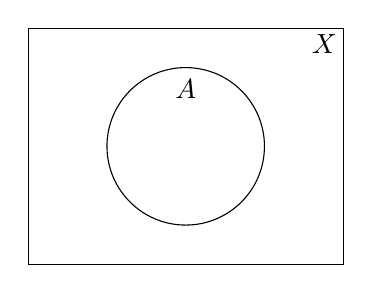
\begin{tikzpicture}

    % 画一个矩形
    \draw[thin] (0,0) rectangle (4,3);

    % 画一个圆形
    \draw[thin] (2,1.5) circle (1);

    % 插入文字
    \node[anchor=north, inner sep=4pt] at (2,2.5) {$A$};
    \node[anchor=north east, inner sep=2pt] at (4,3) {$X$};

  \end{tikzpicture}
\end{figure}

我们可以用维恩图来表示两个集合 $A, B$ 之间三种可能的关系如下。

\begin{figure}[H]
  \centering
  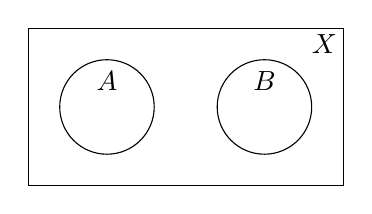
\begin{tikzpicture}

    % 画一个矩形
    \draw[thin] (0,0) rectangle (4,2);

    % 画一个圆形
    \draw[thin] (1,1) circle (0.6);
    \draw[thin] (3,1) circle (0.6);

    % 插入文字
    \node[anchor=north, inner sep=4pt] at (1,1.6) {$A$};
    \node[anchor=north, inner sep=4pt] at (3,1.6) {$B$};
    \node[anchor=north east, inner sep=2pt] at (4,2) {$X$};

  \end{tikzpicture}
  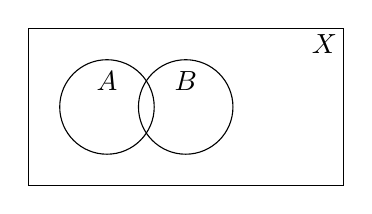
\begin{tikzpicture}

    % 画一个矩形
    \draw[thin] (0,0) rectangle (4,2);

    % 画一个圆形
    \draw[thin] (1,1) circle (0.6);
    \draw[thin] (2,1) circle (0.6);

    % 插入文字
    \node[anchor=north, inner sep=4pt] at (1,1.6) {$A$};
    \node[anchor=north, inner sep=4pt] at (2,1.6) {$B$};
    \node[anchor=north east, inner sep=2pt] at (4,2) {$X$};

  \end{tikzpicture}
  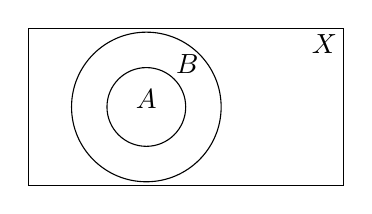
\begin{tikzpicture}

    % 画一个矩形
    \draw[thin] (0,0) rectangle (4,2);

    % 画一个圆形
    \draw[thin] (1.5,1) circle (0.5);
    \draw[thin] (1.5,1) circle (0.95);

    % 插入文字
    \node[anchor=north east, inner sep=2pt] at (2.24,1.74) {$B$};
    \node[anchor=north, inner sep=2pt] at (1.5,1.3) {$A$};
    \node[anchor=north east, inner sep=2pt] at (4,2) {$X$};

  \end{tikzpicture}
\end{figure}%
最左边图示表示的是 $A, B$ 没有共同的元素，中间图示表示的是 $A, B$ 有共同元素但互相没有包含关系，而最右边表示的是 $A \subseteq B$。

有时维恩图可以帮助我们了解一些集合的性质，甚至给我们证明这些性质的提示。例如以下的图示便可以帮助我们理解命题 3.1.4 (2) “若 $A \subseteq B$ 且 $B \subseteq C$，则 $A \subseteq C$” 这个性质。
\begin{figure}[H]
  \centering
  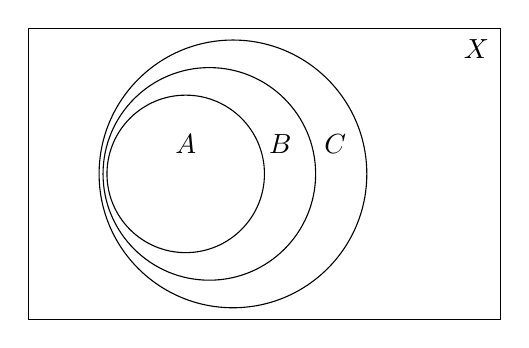
\begin{tikzpicture}

    % 画一个矩形
    \draw[thin] (0,0) rectangle (6,3.7);

    % 画一个圆形
    \draw[thin] (2,1.85) circle (1);
    \draw[thin] (2.3,1.85) circle (1.35);
    \draw[thin] (2.6,1.85) circle (1.7);

    % 插入文字
    \node[anchor=north, inner sep=4pt] at (2,2.5) {$A$};
    \node[anchor=north, inner sep=4pt] at (3.2,2.5) {$B$};
    \node[anchor=north, inner sep=4pt] at (3.9,2.5) {$C$};
    \node[anchor=north east, inner sep=4pt] at (6,3.7) {$X$};

  \end{tikzpicture}
\end{figure}

当然了维恩图只是让我们参考用，绝不能只是画个图就以为证明完成。

\begin{question}
假设 $A, B, C$ 为集合。已知 $A \subseteq B$。若 $B$ 和 $C$ 没有共同的元素，画出可能的维恩图。是否可以确定 $A$ 和 $C$ 没有共同元素？又若 $B$ 和 $C$ 有共同的元素，画出可能的维恩图，是否可确定 $A$ 和 $C$ 有共同元素？同样地，分 $A, C$ 有/没有共同元素的情况，画出可能的维恩图，并探讨是否依此可确定 $B, C$ 有没有共同元素。
\end{question}

最后提醒大家千万不要把 “$\in$”（属于）和 “$\subseteq$”（包含于）弄混淆。“$\in$” 指的是元素和集合之间的关系，而 “$\subseteq$” 指的是两集合间的关系。对于集合我们有 $A \subseteq B$ 且 $B \subseteq C$ 则 $A \subseteq C$ 的性质，但对于元素 $A \in B$ 且 $B \in C$ 未必可得 $A \in C$。例如 $A = \{1\}$, $B = \{\{1\}\}$, $C = \{\{\{1\}\}\}$。我们有 $A \in B$ 且 $B \in C$，但很明显地 $A \notin C$。

\section{集合运算}

所谓集合运算（set operation），\index{集合运算（set operation）}就是利用两个已知的集合得到另一个集合的方法。我们将介绍集合间几种重要的运算，即交集、并集和差集，并探讨这几种集合运算之间重要的性质。

\subsection{交集与并集}

首先我们定义交集与并集。

\begin{definition}
设 $A, B$ 为集合。我们令 $A \cap B = \{x : x \in A \text{ 且 }~ x \in B\}$ 称之为 $A$ 和 $B$ 的{\bf 交集（intersection）}。\index{交集（intersection）}令 $A \cup B = \{x : x \in A \text{ 或 }~ x \in B\}$ 称之为 $A$ 和 $B$ 的{\bf 并集（union）}\index{并集（union）}。
\end{definition}

简单地说 $A \cap B$ 就是将 $A, B$ 共同的元素收集起来所得的集合，而 $A \cup B$ 是将 $A, B$ 所有的元素收集起来而得的集合。例如以下的例子。

\begin{example}
令 $A = \{1, 2, 3\}$, $B = \{2, 4, 6\}$。由于只有 $2$ 是同时属于 $A$ 且属于 $B$，所以得 $A \cap B = \{2\}$。而 $1, 3$ 虽没有在 $B$ 但都属于 $A$，符合属于 $A$ 或属于 $B$ 的条件，故知 $1, 3$ 皆属于 $A \cup B$。同理 $4, 6$ 亦属于 $A \cup B$。至于 $2$，既然同时属于 $A$ 和 $B$，当然符合属于 $A$ 或属于 $B$ 的条件，故知 $2$ 也属于 $A \cup B$。又由于没有其他的数在 $A$ 中或 $B$ 中，我们可以确定 $A \cup B = \{1, 2, 3, 4, 6\}$。
\end{example}

并集和交集与原来的集合是有关系的。例如在上面的例子中我们有 $A \cap B = \{2\} \subseteq A = \{1, 2, 3\}$ 以及 $B = \{2, 4, 6\} \subseteq A \cup B = \{1, 2, 3, 4, 6\}$。事实上，若 $x \in A \cap B$，表示 $x \in A$ 且 $x \in B$，故知 $x$ 一定属于 $A$ 且 $x$ 一定属于 $B$，所以我们有
\begin{equation}
(A \cap B) \subseteq A \quad \text{和} \quad (A \cap B) \subseteq B.
\end{equation}
注意 $A \cap B$ 有可能是空集，此时我们称 $A, B$ 为\textbf{不相交（disjoint）}。\index{不相交（disjoint）}不过空集包含于任意的集合，所以当 $A, B$ 为不相交时上式仍然成立。另一方面若 $x \in A$，则 $x$ 必属于 $A$ 或 $B$，所以 $x \in A \cup B$ 成立。我们有
\begin{equation}
A \subseteq (A \cup B) \quad \text{和} \quad B \subseteq (A \cup B).
\end{equation}

\begin{question}
试证明 $(A \cap A) = A$ 以及 $(A \cup A) = A$。
\end{question}

交集和并集在某种程度上可以说是保持包含关系的，事实上我们有以下的性质。

\begin{proposition}
设 $A, B, C, D$ 皆为集合，满足 $A \subseteq B$ 且 $C \subseteq D$。则
$$ (A \cap C) \subseteq (B \cap D) \quad \text{和} \quad (A \cup C) \subseteq (B \cup D). $$
\end{proposition}

\begin{proof}
因 $A \subseteq B$，可由 $x \in A$ 得 $x \in B$。同理因 $C \subseteq D$，可由 $x \in C$ 得 $x \in D$。现若 $x \in A \cap C$，表示 $x \in A$ 且 $x \in C$，故可得 $x \in B$ 且 $x \in D$。得证 $(A \cap C) \subseteq (B \cap D)$。同理，若 $x \in A \cup C$，表示 $x \in A$ 或 $x \in C$。当 $x \in A$ 时可得 $x \in B$，而当 $x \in C$ 时可得 $x \in D$。故由 $x \in A \cup C$ 可得 $x \in B \cup D$。得证 $(A \cup C) \subseteq (B \cup D)$。
\end{proof}

特别地，当 $A \subseteq B$ 且 $A \subseteq D$ 时，我们可以考虑 $C = A$ 的情形套用命题 3.2.3 得 $(A \cap A) \subseteq (B \cap D)$。又由于 $(A \cap A) = A$，得知 $A \subseteq (B \cap D)$。同理，当 $A \subseteq B$ 且 $C \subseteq B$ 时，我们有 $(A \cup C) \subseteq (B \cup B)$。又由于 $(B \cup B) = B$，得知 $(A \cup C) \subseteq B$。我们证得以下性质。既然这个结果是由命题 3.2.3 简单推导而得，我们就用推论 （corollary）称之。

\begin{corollary}
假设 $A, B, C, D, E$ 为集合。
\begin{enumerate}
  \item 若 $A \subseteq B$ 且 $A \subseteq C$，则 $A \subseteq (B \cap C)$。
  \item 若 $D \subseteq A$ 且 $E \subseteq A$，则 $(D \cup E) \subseteq A$。
\end{enumerate}
\end{corollary}

\begin{question}
试直接证明推论 3.2.4，并用此结果推导出命题 3.2.3。
\end{question}

我们也可利用交集或并集来判断两集合的包含关系。我们有以下的结果。

\begin{proposition}
假设 $A, B$ 为集合。则以下是等价的。
\begin{enumerate}[label={(\arabic*)}]
  \item $A \subseteq B$。
  \item $(A \cap B) = A$。
  \item $(A \cup B) = B$。
\end{enumerate}
\end{proposition}

\begin{proof}
我们证明 (1) $\Leftrightarrow$ (2) 以及 (1) $\Leftrightarrow$ (3)。

(1) $\Leftrightarrow$ (2)：假设 $A \subseteq B$，我们要证明 $(A \cap B) = A$。事实上由式子 (3.1) 我们知 $(A \cap B) \subseteq A$，故仅要证明 $A \subseteq (A \cap B)$。然而已知 $A \subseteq A$ 以及 $A \subseteq B$，故由推论 3.2.4 得 $A \subseteq (A \cap B)$。因此证明了 (1) $\Rightarrow$ (2)。另一方面，由式子 (3.1) 我们知 $(A \cap B) \subseteq B$。故由 $A = (A \cap B)$ 可得 $A \subseteq B$，证明了 (2) $\Rightarrow$ (1)。

(1) $\Leftrightarrow$ (3)：假设 $A \subseteq B$，我们要证明 $(A \cup B) = B$。事实上由式子 (3.2) 我们知 $B \subseteq (A \cup B)$，故仅要证明 $(A \cup B) \subseteq B$。然而已知 $A \subseteq B$ 以及 $B \subseteq B$，故由推论 3.2.4，得 $(A \cup B) \subseteq B$。因此证明了 (1) $\Rightarrow$ (3)。另一方面，由式子 (3.2) 我们知 $A \subseteq (A \cup B)$。故由 $(A \cup B) = B$ 可得 $A \subseteq B$，证明了 (3) $\Rightarrow$ (1)。
\end{proof}

由定义我们知道 “交集” 和逻辑的 “且” 有关，而 “并集” 和 “或” 有关。所以我们很容易推得以下的关系：
\begin{enumerate}[label={(\arabic*)}]
  \item $A \cap B = B \cap A$。
  \item $A \cup B = B \cup A$。
  \item $(A \cap B) \cap C = A \cap (B \cap C)$。
  \item $(A \cup B) \cup C = A \cup (B \cup C)$。
\end{enumerate}
由于 (3) 的关系，以后多个集合的交集我们便省略括弧不必去强调哪几个先作交集，例如直接写成 $A \cap B \cap C$。同理由于 (4)，以后多个集合的并集我们也省略括弧，例如直接写成 $A \cup B \cup C$。

利用逻辑 $\wedge, \vee$ 之间的分配性质，即
$$ ((P \wedge Q) \vee R) \sim ((P \vee R) \wedge (Q \vee R)), $$
$$ ((P \vee Q) \wedge R) \sim ((P \wedge R) \vee (Q \wedge R)), $$
我们有以下的性质。

\begin{proposition}
假设 $A, B, C$ 为集合，则
$$ ((A \cap B) \cup C) = (A \cup C) \cap (B \cup C), $$
$$ ((A \cup B) \cap C) = (A \cap C) \cup (B \cap C). $$
\end{proposition}

\begin{proof}
首先由 $(A \cap B) \subseteq A$ 以及 $C \subseteq C$ 利用命题 3.2.3 得 $((A \cap B) \cup C) \subseteq (A \cup C)$。同理知 $((A \cap B) \cup C) \subseteq (B \cup C)$。再利用推论 3.2.4 得 $((A \cap B) \cup C) \subseteq (A \cup C) \cap (B \cup C)$。另一方面假设 $x \in (A \cup C) \cap (B \cup C)$ 表示 $x \in A \cup C$ 且 $x \in B \cup C$。我们利用分类讨论，考虑 $x \in C$ 和 $x \notin C$ 这两种情况。若 $x \in C$，则当然 $x \in (A \cap B) \cup C$。而若 $x \notin C$，则由 $x \in A \cup C$ 且 $x \in B \cup C$，知 $x \in A$ 且 $x \in B$，亦即 $x \in A \cap B$。故此时仍有 $x \in (A \cap B) \cup C$。也就是说不管哪种情况，我们都可以由 $x \in (A \cup C) \cap (B \cup C)$ 推得 $x \in (A \cap B) \cup C$，得证 $((A \cup C) \cap (B \cup C)) \subseteq (A \cap B) \cup C$。故知 $((A \cap B) \cup C) = (A \cup C) \cap (B \cup C)$。

至于 $((A \cup B) \cap C) = (A \cap C) \cup (B \cap C)$ 的证明，首先由 $A \subseteq (A \cup B)$ 以及 $C \subseteq C$ 利用命题 3.2.3 得 $(A \cap C) \subseteq ((A \cup B) \cap C)$，同理我们有 $(B \cap C) \subseteq ((A \cup B) \cap C)$。故由推论 3.2.4 知 $(A \cap C) \cup (B \cap C) \subseteq ((A \cup B) \cap C)$。另一方面，若 $x \in (A \cup B) \cap C$，表示 $x \in A \cup B$ 且 $x \in C$。由 $x \in A \cup B$，我们知 $x \in A$ 或 $x \in B$。当 $x \in A$ 时，由于已知 $x \in C$，故得 $x \in A \cap C$。此时自然有 $x \in (A \cap C) \cup (B \cap C)$。同理，当 $x \in B$ 时，可得 $x \in B \cap C$。因此也有 $x \in (A \cap C) \cup (B \cap C)$，得证 $((A \cup B) \cap C) \subseteq (A \cap C) \cup (B \cap C)$。故知 $((A \cup B) \cap C) = (A \cap C) \cup (B \cap C)$。
\end{proof}

\begin{question}
试利用命题 3.2.5 中 (1) $\Rightarrow$ (2) 的结果以及命题 3.2.6 证明命题 3.2.5 中 (2) $\Rightarrow$ (3)。
\end{question}

\subsection{差集}

我们定义何谓差集。

\begin{definition}
假设 $A, B$ 为集合，定义 $A \setminus B = \{x : x \in A \text{ 且 }~ x \notin B\}$，称之为 $B$ 在 $A$ 中的{\bf 差集（set difference）}。\index{差集（set difference）}若 $X$ 为全集，则令 $A^c = X \setminus A = \{x : x \notin A\}$ 称之为 $A$ 的{\bf 补集（complement）}\index{补集（complement）}。
\end{definition}

注意 $A^c$ 的定义原本应为 $\{x : x \in X \text{ 且 }~ x \notin A\}$，但因 $X$ 为全集，我们知道所有元素皆在 $X$ 中，故省略 $x \in X$ 直接写 $x \notin A$。所以在使用补集时要特别注意是否已明确说明了什么是全集，否则会有符号不唯一的问题。例如若 $\mathbb{Q}$ 为全集，则 $\mathbb{Q}^c = \emptyset$，而当全集为 $\mathbb{R}$ 时，$\mathbb{Q}^c$ 就是所有无理数所成的集合了。

利用补集的符号，依定义我们有 $A \setminus B = A \cap B^c$，从这里我们知道一般情况下 $A \setminus B$ 和 $B \setminus A$ 是不相同的。事实上我们有 $(A \setminus B) \cap (B \setminus A) = \emptyset$。这是因为很明显地 $A \cap A^c = \emptyset$ 且 $B \cap B^c = \emptyset$，故知
$$ (A \setminus B) \cap (B \setminus A) = (A \cap B^c) \cap (B \cap A^c) = (A \cap A^c) \cap (B \cap B^c) = \emptyset. $$

\begin{example}
假设 $X = \{1, 2, 3, 4, 5, 6\}$, $A = \{1, 2, 3\}$, $B = \{2, 4, 6\}$。因 $1, 3 \in A$ 且 $1 \notin B$ 且 $3 \notin B$，知 $1, 3 \in A \setminus B$。虽然 $2 \in A$ 但是 $2 \in B$，故 $2 \notin A \setminus B$。得 $A \setminus B = \{1, 3\}$。同理可得 $B \setminus A = \{4, 6\}$。我们有 $(A \setminus B) \cap (B \setminus A) = \{1, 3\} \cap \{4, 6\} = \emptyset$。又 $1, 3, 5 \in X$ 且 $1, 3, 5$ 皆不在 $B$ 中，故知 $1, 3, 5 \in B^c$。而 $2, 4, 6 \in B$ 故 $2, 4, 6$ 皆不属于 $B^c$，得 $B^c = \{1, 3, 5\}$。最后考虑 $A \cap B^c$ 得 $A \cap B^c = \{1, 2, 3\} \cap \{1, 3, 5\} = \{1, 3\} = A \setminus B$。
\end{example}

接下来我们看差集的一些性质，其实这些性质我们可以用元素的方式证明，不过在证明时由于常出现否定的问题所以经常要用反证法，如此反反复复，容易搞混。但如使用补集符号，就可以化繁为简。所以我们先介绍有关于补集的一些性质，再处理差集的问题。

\begin{proposition}
假设 $A, B$ 为集合，我们有以下的性质。
\begin{enumerate}[label={(\arabic*)}]
  \item $(A^c)^c = A$。
  \item $(A \cap B)^c = (A^c \cup B^c)$。
  \item $(A \cup B)^c = (A^c \cap B^c)$。
  \item $A \subseteq B$ 当且仅当 $B^c \subseteq A^c$。
\end{enumerate}
\end{proposition}

\begin{proof}
这些性质都可以利用前面逻辑相关的等价推导。我们主要使用的方式就是 $x \notin A$ 是 $x \in A$ 的否定，所以
$$ (x \in A^c) \sim (x \notin A)\sim \neg(x \in A). $$

(1) $x \in (A^c)^c$ 表示 $x \notin A^c$，即 $\neg(x \in A^c)$。等同于 $\neg(x \notin A)$，亦即 $\neg(\neg(x \in A))$。因此由式子(1.7)知此与 $x \in A$ 等价，故得证。

(2) $x \in (A \cap B)^c \sim \neg(x \in (A \cap B)) \sim \neg((x \in A) \wedge (x \in B))$。由式子(1.8)知此与 $\neg(x \in A) \vee \neg(x \in B)$ 等价，亦即 $(x \in A^c) \vee (x \in B^c)$，故得证等同于 $x \in (A^c \cup B^c)$。

(3) $x \in (A \cup B)^c \sim \neg(x \in (A \cup B)) \sim \neg((x \in A) \vee (x \in B))$。由式子(1.9)知此与 $\neg(x \in A) \wedge \neg(x \in B)$ 等价，亦即 $(x \in A^c) \wedge (x \in B^c)$，故得证等同于 $x \in (A^c \cap B^c)$。

(4) 由于 $A \subseteq B$ 等价于 $(x \in A) \Rightarrow (x \in B)$，且 $B^c \subseteq A^c$ 等价于 $\neg(x \in B) \Rightarrow \neg(x \in A)$。由式子(1.11)我们有$((x \in A) \Rightarrow (x \in B)) \sim (\neg(x \in B) \Rightarrow \neg(x \in A))$，故得证。
\end{proof}

利用命题 3.2.9，我们立即可得以下的定理。

\begin{corollary}
假设 $A, B, C$ 为集合，我们有以下的性质。
\begin{enumerate}[label={(\arabic*)}]
  \item $(C \setminus (C \setminus A)) = (C \cap A)$。
  \item $C \setminus (A \cap B) = (C \setminus A) \cup (C \setminus B)$。
  \item $C \setminus (A \cup B) = (C \setminus A) \cap (C \setminus B)$。
  \item 若 $A \subseteq B$ 则 $(C \setminus B) \subseteq (C \setminus A)$。
\end{enumerate}
\end{corollary}

\begin{proof}
我们使用补集、交集、并集之间的关系证明。

(1) 依定义 $(C \setminus (C \setminus A)) = C \cap (C \setminus A)^c = C \cap (C \cap A^c)^c$。由命题 3.2.9 (1)(2)，$(C \cap A^c)^c = C^c \cup (A^c)^c = C^c \cup A$，故得 $(C \setminus (C \setminus A)) = C \cap (C^c \cup A)$。再由分配律
$$ C \cap (C^c \cup A) = (C \cap C^c) \cup (C \cap A) = \emptyset \cup (C \cap A) $$
得证 $(C \setminus (C \setminus A)) = (C \cap A)$。

(2) 依定义 $C \setminus (A \cap B) = C \cap (A \cap B)^c$。由命题 3.2.9 (2)，$(A \cap B)^c = (A^c \cup B^c)$，故得 $C \setminus (A \cap B) = C \cap (A^c \cup B^c)$。再由分配律 $C \cap (A^c \cup B^c) = (C \cap A^c) \cup (C \cap B^c)$。得证 $C \setminus (A \cap B) = (C \setminus A) \cup (C \setminus B)$。

(3) 依定义 $C \setminus (A \cup B) = C \cap (A \cup B)^c$。由命题 3.2.9 (3)，$(A \cup B)^c = (A^c \cap B^c)$，故得 $C \setminus (A \cup B) = C \cap (A^c \cap B^c)$。再由 $C \cap (A^c \cap B^c) = (C \cap A^c) \cap (C \cap B^c)$。得证 $C \setminus (A \cup B) = (C \setminus A) \cap (C \setminus B)$。

(4) 依定义 $C \setminus B = C \cap B^c$。现若 $A \subseteq B$ 由命题 3.2.9 (4) 可得 $B^c \subseteq A^c$，故得 $C \cap B^c \subseteq C \cap A^c$，得证 $(C \setminus B) \subseteq (C \setminus A)$。
\end{proof}

推论 3.2.10 (4) 的反向是不正确的，不过我们有以下之结果。

\begin{proposition}
假设 $A, B, C$ 为集合。$(C \cap A) \subseteq (C \cap B)$ 当且仅当 $(C \setminus B) \subseteq (C \setminus A)$。
特别地，若已知 $A \subseteq C$，则 $A \subseteq B$ 当且仅当 $(C \setminus B) \subseteq (C \setminus A)$。
\end{proposition}

\begin{proof}
首先注意 $C \setminus A = C \setminus (C \cap A)$，这是因为由推论 3.2.10 (2)，
$$ C \setminus (C \cap A) = (C \setminus C) \cup (C \setminus A) = \emptyset \cup (C \setminus A) = C \setminus A. $$
同理 $C \setminus B = C \setminus (C \cap B)$。

现若 $(C \cap A) \subseteq (C \cap B)$，利用推论 3.2.10 (4) 可得 $C \setminus (C \cap B) \subseteq C \setminus (C \cap A)$，得证 $(C \setminus B) \subseteq (C \setminus A)$。反之，若 $(C \setminus B) \subseteq (C \setminus A)$，则同样由推论 3.2.10 (4) 得 $C \setminus (C \setminus A) \subseteq C \setminus (C \setminus B)$。再由命题 3.2.10 (1) 得证 $(C \cap A) \subseteq (C \cap B)$。

由推论 3.2.10 (4) 已知若 $A \subseteq B$ 则 $(C \setminus B) \subseteq (C \setminus A)$。故当已知 $A \subseteq C$，我们仅要证明：若 $(C \setminus B) \subseteq (C \setminus A)$ 则 $A \subseteq B$。此时由前知 $(C \setminus B) \subseteq (C \setminus A)$ 可得 $(C \cap A) \subseteq (C \cap B)$。故由 $A \subseteq C$ 的假设得 $A = (C \cap A) \subseteq (C \cap B)$。但 $(C \cap B) \subseteq B$，故得证 $A \subseteq B$。
\end{proof}

\begin{question}
$C \setminus (B \setminus A)$ 会等于 $(C \setminus B) \setminus A$ 吗？试证明 $C \setminus (B \setminus A) = (C \setminus B) \cup (C \cap A)$ 以及 $(C \setminus B) \setminus A = C \setminus (B \cup A)$。
\end{question}

其实这些集合运算之间的关系与性质，都可以直接各边取一元素，利用第一章所介绍逻辑联结词的性质得到集合包含关系，最后证得两边集合相等。另一方面我们也可套用这一章中所介绍各集合的运算的性质推导。这两者方法并无好坏之分，虽然有时直接套用集合运算的性质推导很快速，但它并非万能。在这里我们并不是鼓励大家用背诵的方式记忆这么多的性质，而是希望大家能够学习如何利用一些已知的性质推导出新的定理。最后我们再看一个例子。

\begin{example}
假设 $A, B, C$ 为集合且 $B^c \subseteq A$，我们要证明 $((C \setminus A) \cup B) = B$。
\end{example}

方法一：我们用元素的方法处理。首先已知 $B \subseteq ((C \setminus A) \cup B)$，故要证明等式成立只要证明 $((C \setminus A) \cup B) \subseteq B$。现假设 $x \in ((C \setminus A) \cup B)$，我们要证明 $x \in B$。然而 $x \in ((C \setminus A) \cup B)$ 表示 $x \in C \setminus A$ 或 $x \in B$。如果 $x \in B$，则证明结束，所以我们仅要讨论 $x \in C \setminus A$ 的情形，即 $x \in C$ 且 $x \notin A$。因为无法直接证明 $x \in B$，所以我们可以考虑反证法，即假设 $x \notin B$ 而得到矛盾。现若 $x \notin B$，表示 $x \in B^c$，故由 $B^c \subseteq A$ 的假设得 $x \in A$。此与 $x \notin A$ 相矛盾，故知 $x \in B$。得证 $((C \setminus A) \cup B) \subseteq B$。

方法二：我们也可完全用前面证得的性质处理。首先看到等式左右两边都有 $B$，所以我们可以利用命题 3.2.5。也就是说若能证明 $(C \setminus A) \subseteq B$，则可得证 $((C \setminus A) \cup B) = B$。如何证明 $(C \setminus A) \subseteq B$ 呢？由于 $(C \setminus A) \subseteq C$，利用命题 3.2.11，我们只要验证 $(C \setminus B) \subseteq (C \setminus (C \setminus A))$。然而左边 $C \setminus B = C \cap B^c$，右边 $C \setminus (C \setminus A) = C \cap A$，所以由 $B^c \subseteq A$ 得证 $(C \setminus B) \subseteq (C \setminus (C \setminus A))$，因而得 $(C \setminus A) \subseteq B$。

\section{加标集族}

在前一节中，我们谈交集或并集时，是将其视为两个集合间的运算。不过当我们知道交集和并集有所谓的结合律后，我们便可以谈论多个集合的并集与交集了。这一节中，我们藉由适当的符号与定义的推广，将探讨任意多个集合的并集与交集问题。大致上之前谈的两个集合的交集与并集的性质，都可以推广到更一般的情形。不过处理无限多个集合的情况，有些地方可能和有限的情况稍有不同，要特别留意。

当我们谈论有限多个集合的交集和并集时，如果集合个数不多，例如 5 个集合 $A, B, C, D, E$ 的交集，我们直接用 $A \cap B \cap C \cap D \cap E$ 来表示。这里我们都可以不用括弧区分到底哪两个集合先交集后再和其他的集合做交集，因为交集有结合律。我们也不必担心交集的顺序，因为交集有交换性。同样地对于并集也是如此。当集合的个数太多时，像前面这样一一列出就不切实际了。遇到这种情形，我们可以把要处理的集合一一编号，例如有 100 个集合，我们就编成 $A_1, A_2, \dots, A_{100}$（当然了，这些 $A_i$ 是什么应说明清楚）。然后这些集合的交集与并集我们便像处理加法的求和（summation）符号，将这些集合的交集与并集分别用 $\bigcap_{i=1}^{100} A_i$，$\bigcup_{i=1}^{100} A_i$ 来表示。例如若 $A_i = [i-1, i]$（即介于 $i-1$ 和 $i$ 之间的实数），则 $\bigcap_{i=1}^{100} A_i = \emptyset$，$\bigcup_{i=1}^{100} A_i = [0, 100]$。

如果有无穷多集合怎么办？像前面的例子，如果对所有的自然数 $i \in \mathbb{N}$，$A_i$ 皆有定义，我们可以考虑对所有的 $A_i$ 的交集和并集。这时候我们一般可以学无穷级数的方法，将这些交集和并集分别表示成 $\bigcap_{i=1}^{\infty} A_i$，$\bigcup_{i=1}^{\infty} A_i$。当然了，这样的符号底下表示的是 $i$ 从哪一个数开始，上面表示的是到哪一个为止，所以我们要考虑 $A_5, A_6, A_7, A_8$ 的交集和并集就可以分别用 $\bigcap_{i=5}^{8} A_i$，$\bigcup_{i=5}^{8} A_i$ 来表示。因此一般若要谈 $i$ 从 $m$ 到 $n$ 的 $A_i$ 之交集与并集，我们便分别用 $\bigcap_{i=m}^{n} A_i$，$\bigcup_{i=m}^{n} A_i$ 来表示。而要表达所有 $i$ 大于等于 $m$ 的 $A_i$ 之交集与并集，我们便分别用 $\bigcap_{i=m}^{\infty} A_i$，$\bigcup_{i=m}^{\infty} A_i$ 来表示。这里要注意，很多同学会误以为 $\bigcap_{i=m}^{\infty} A_i$，$\bigcup_{i=m}^{\infty} A_i$ 是 $\bigcap_{i=m}^{n} A_i$，$\bigcup_{i=m}^{n} A_i$ 当 $n$ 趋近于 $\infty$ 的极限。这个说法是有问题的，因为我们从未定义过 “集合的极限”。

不过这些符号仍不够我们的需求。有时我们要探讨的集合，它们的个数是不能像整数一样一个一个数的。例如实数，就无法一个一个数。所以若我们谈的集合和实数有关，如 $(-r, r)$ 其中 $r > 0$这样的区间，要如何表达所有这样的区间的交集与并集呢？于是乎，我们引进了\textbf{指标集（index set）}\index{指标集（index set）}的概念。所谓指标集就是你要用来 “编码” 的东西所成的集合。例如前面 $A_i = [i-1, i]$ 的例子，我们考虑的 $i$ 是所有的自然数 $\mathbb{N}$，所以此时 $\mathbb{N}$ 便是我们的指标集。而若要探讨 $[-r, r]$ 的情形，我们可以用正实数 $\mathbb{R}^+$ 为我们的指标集，将要考虑的区间编码成 $A_r = [-r, r]$。这样将所有被编码好的集合 $A_r, r \in \mathbb{R}^+$ 收集在一起，便是所谓的\textbf{加标集族（indexed family）}\index{加标集族（indexed family）}了。所以一般来说，我们要先说好指标集是什么集合，接下来要说明要探讨的集合如何用指标集里的元素编码，这样才能形成一个加标集族。也就是说若 $I$ 为指标集，我们必须说明 $A_i$ 是什么，这样 $\{A_i, i \in I\}$ 便会是一个加标集族。

接下来，我们便是要定义一个加标集族里的集合的交集与并集。注意，即使只有有限个集合，我们仍可将其视为加标集族。例如两个集合 $A, B$，我们仍可将其视为指标集为 $I = \{1, 2\}$ 的加标集族，其中 $A_1 = A, A_2 = B$。所以我们定义加标集族的交集与并集需与有限集合的交集与并集一致。当我们有两个集合 $A, B$ 时，要求交集的元素必须在每一个集合中；而并集里的元素需在 $A, B$ 某一个中。所以我们有以下的定义。

\begin{definition}
假设 $I$ 为指标集，而 $\{A_i, i \in I\}$ 为以 $I$ 为指标集的加标集族。
定义此加标集族的交集\index{交集（intersection）!加标集族的$\sim$（of indexed family）}为
$$ \bigcap_{i \in I} A_i = \{x : x \in A_i, \forall i \in I\}. $$
定义此加标集族的并集\index{并集（union）!加标集族的$\sim$（of indexed family）}为
$$ \bigcup_{i \in I} A_i = \{x : x \in A_i, \exists i \in I\}. $$
\end{definition}

利用此定义，我们看以下的例子。

\begin{example}
考虑指标集 $I$ 为大于 $1$ 的整数。对任意 $i \in I$，令 $A_i = \{m/i : m \in \mathbb{Z}\}$。我们要证明
$$ \bigcap_{i \in I} A_i = \mathbb{Z}, \quad \bigcup_{i \in I} A_i = \mathbb{Q}. $$
\end{example}
首先，任意 $n \in \mathbb{Z}$，我们都可以写成 $n = ni/i$。由于 $ni \in \mathbb{Z}$，故得 $n \in A_i, \forall i \in I$。得证 $\mathbb{Z} \subseteq \bigcap_{i \in I} A_i$。另一方面，若 $x \in \bigcap_{i \in I} A_i$，表示对任意 $i \in I$ 皆有 $x \in A_i$。现由于 $x \in A_2$ 以及 $x \in A_3$，我们有 $x = m/2$ 且 $x = m'/3$，其中 $m, m' \in \mathbb{Z}$。然而此即表示 $3m = 2m'$，故知 $3m$ 必为偶数。因而得知 $m$ 为偶数 $2n$，其中 $n \in \mathbb{Z}$。代回得 $x = m/2 = n \in \mathbb{Z}$。得证 $\bigcap_{i \in I} A_i \subseteq \mathbb{Z}$，故 $\bigcap_{i \in I} A_i = \mathbb{Z}$。

现若 $x \in \mathbb{Q}$，依有理数之定义，$x$ 可写成 $m/n$，其中 $m \in \mathbb{Z}, n \in \mathbb{N}$。现若 $n = 1$，即 $x = m \in \mathbb{Z}$。我们可以将 $x$ 写成 $x = 2m/2$，知此时 $x \in A_2$。而若 $n \geq 2$，表示 $n \in I$，故此时 $x \in A_n$。得证 $\mathbb{Q} \subseteq \bigcup_{i \in I} A_i$。另一方面，若 $x \in \bigcup_{i \in I} A_i$，表示存在 $n \in I$，使得 $x \in A_n$。故依定义得 $x = m/n$，其中 $m \in \mathbb{Z}$。此即表示 $x \in \mathbb{Q}$，得证 $\bigcup_{i \in I} A_i \subseteq \mathbb{Q}$，故 $\bigcup_{i \in I} A_i = \mathbb{Q}$。

\begin{question}
令 $A_i$ 如例 3.3.2 所设。利用当 $m \in \mathbb{Z}$ 时，若 $p, q$ 为两互质整数且 $p$ 整除 $mq$，则 $p$ 整除 $m$ 之事实，证明若 $p, q$ 为两互质整数，则 $A_p \cap A_q = \mathbb{Z}$。依此证明当 $m \in \mathbb{N}$，$\bigcap_{i=m}^{\infty} A_i = \mathbb{Z}$。
\end{question}

现在我们探讨一些有关两集合的交集与并集的性质，是否可以推广到更一般加标集族的情形。首先命题 3.2.3 是可以推广的。

\begin{proposition}
假设 $\{A_i, i \in I\}$, $\{B_i, i \in I\}$ 是以 $I$ 为指标集的两组加标集族。若对于所有 $i \in I$ 皆有 $A_i \subseteq B_i$，则
$$ \bigcap_{i \in I} A_i \subseteq \bigcap_{i \in I} B_i \quad \text{且} \quad \bigcup_{i \in I} A_i \subseteq \bigcup_{i \in I} B_i. $$
\end{proposition}

\begin{proof}
设 $x \in \bigcap_{i \in I} A_i$，表示对所有 $i \in I$，皆有 $x \in A_i$，故由 $A_i \subseteq B_i$，得 $x \in B_i$。因为这是对任意的 $i \in I$ 皆成立，故得 $x \in \bigcap_{i \in I} B_i$。得证 $\bigcap_{i \in I} A_i \subseteq \bigcap_{i \in I} B_i$。

现若 $x \in \bigcup_{i \in I} A_i$，表示存在 $i \in I$ 使得 $x \in A_i$，故由 $A_i \subseteq B_i$，得 $x \in B_i$。此即表示 $x \in \bigcup_{i \in I} B_i$，得证 $\bigcup_{i \in I} A_i \subseteq \bigcup_{i \in I} B_i$。
\end{proof}

很容易知道，若对于任意 $i \in I$，皆有 $A_i = A$，则 $\bigcap_{i \in I} A_i = A$ 且 $\bigcup_{i \in I} A_i = A$。所以我们套用命题 3.3.3，有以下推论 3.2.4 的推广。

\begin{corollary}
假设 $A, B$ 为集合且 $\{A_i, i \in I\}$, $\{B_i, i \in I\}$ 是以 $I$ 为指标集的加标集族。
\begin{enumerate}
  \item 若对于所有 $i \in I$ 皆有 $A \subseteq A_i$，则 $A \subseteq \bigcap_{i \in I} A_i$。
  \item 若对于所有 $i \in I$ 皆有 $B_i \subseteq B$，则 $\bigcup_{i \in I} B_i \subseteq B$。
\end{enumerate}
\end{corollary}

虽然前面几个结果显示一些关于有限多个集合的交集或并集的性质可以推广到无穷多个集合的交集或并集，不过这并不是完全对的。例如有可能有一些集合当你在它们中任意取有限多个做交集时都不是空集，但是取无穷多个做交集时有可能会是空集。我们有以下的例子。

\begin{example}
我们要举例说明有可能一个以自然数 $\mathbb{N}$ 为指标集的加标集族 $\{A_i, i \in I\}$，满足对所有 $n \in \mathbb{N}$ 皆有 $\bigcap_{i=1}^{n} A_i$ 不是空集（甚至会有无穷多个元素），但 $\bigcap_{i=1}^{\infty} A_i$ 是空集。

事实上对所有 $i \in \mathbb{N}$ 考虑 $A_i$ 为开区间 $(i, \infty)$。此时 $A_i$ 满足 $A_i \neq \emptyset$ 且当 $j \geq i$ 时，$A_j \subseteq A_i$。因此得 $\bigcap_{i=1}^{n} A_i = A_n = (n, \infty) \neq \emptyset$。但 $\bigcap_{i=1}^{\infty} A_i = \emptyset$。这是因为若 $x \in \bigcap_{i=1}^{\infty} A_i$，则因 $x \in \mathbb{R}$ 必存在 $n \in \mathbb{N}$ 满足 $n > x$。我们得 $x \notin A_n = (n, \infty)$。此与 $x \in \bigcap_{i=1}^{\infty} A_i$ 相矛盾，得证 $\bigcap_{i=1}^{\infty} A_i = \emptyset$。
\end{example}

从上面这个例子我们知道，一些在有限多个集合的交集或并集会对的情形，在无穷多个集合的时候有可能是错的，所以还是要多加留意。

\begin{question}
假设 $A_i$ 为例 3.3.5 中的开区间 $(i, \infty)$，为何不是 $\bigcap_{i=1}^{\infty} A_i = \{\infty\}$？
\end{question}

关于交集与并集分配律的性质，我们有以下命题 3.2.6 的推广。

\begin{proposition}
假设 $B$ 为集合，且 $\{A_i, i \in I\}$ 是以 $I$ 为指标集的加标集族。则
$$ \left( \bigcap_{i \in I} A_i \right) \cup B = \bigcap_{i \in I} (A_i \cup B) \quad \text{且} \quad \left( \bigcup_{i \in I} A_i \right) \cap B = \bigcup_{i \in I} (A_i \cap B). $$
\end{proposition}

\begin{proof}
由于对所有 $k \in I$ 皆有 $(\bigcap_{i \in I} A_i) \subseteq (A_k \cup B)$ 且 $B \subseteq (A_k \cup B)$，由推论 3.2.4 (2) 知 $((\bigcap_{i \in I} A_i) \cup B) \subseteq (A_k \cup B)$。因为这是对任意 $k \in I$ 皆对，故由推论 3.3.4 (1) 知
$ \left( \left( \bigcap_{i \in I} A_i \right) \cup B \right) \subseteq \bigcap_{i \in I} (A_i \cup B). $

另一方面，若 $x \in \bigcap_{i \in I} (A_i \cup B)$，则对所有 $i \in I$，皆有 $x \in A_i$ 或 $x \in B$。我们分 $x \in B$ 以及 $x \notin B$ 两种情况来讨论。若 $x \in B$，则自然有 $x \in (\bigcap_{i \in I} A_i) \cup B$。而若 $x \notin B$，则知 $x \in A_i$ 且由于这是对所有 $i \in I$ 皆成立，故得 $x \in \bigcap_{i \in I} A_i$，因此 $x \in (\bigcap_{i \in I} A_i) \cup B$。得证 $\bigcap_{i \in I} (A_i \cup B) \subseteq ((\bigcap_{i \in I} A_i) \cup B)$，故 $(\bigcap_{i \in I} A_i) \cup B = \bigcap_{i \in I} (A_i \cup B)$。

同理，对所有 $k \in I$ 皆有 $(A_k \cap B) \subseteq (\bigcup_{i \in I} A_i)$ 且 $(A_k \cap B) \subseteq B$，由推论 3.2.4 (1) 知 $(A_k \cap B) \subseteq (\bigcup_{i \in I} A_i) \cap B$。因为这是对任意 $k \in I$ 皆对，故由推论 3.3.4 (2) 知
$ \bigcup_{i \in I} (A_i \cap B) \subseteq \left( \bigcup_{i \in I} A_i \right) \cap B. $

另一方面，若 $x \in (\bigcup_{i \in I} A_i) \cap B$，表示 $x \in \bigcup_{i \in I} A_i$ 且 $x \in B$。因此存在 $i \in I$，使得 $x \in A_i$ 且 $x \in B$。亦即存在 $i \in I$ 使得 $x \in A_i \cap B$。故知此时 $x \in \bigcup_{i \in I} (A_i \cap B)$，得证 $((\bigcup_{i \in I} A_i) \cap B) \subseteq \bigcup_{i \in I} (A_i \cap B)$，故 $(\bigcup_{i \in I} A_i) \cap B = \bigcup_{i \in I} (A_i \cap B)$。
\end{proof}

最后我们推广有限集合差集的德摩根定律\index{德摩根定律（DeMorgan's laws）}（命题 3.2.9 (2)(3)）。

\begin{proposition}
假设 $C$ 为集合且 $\{A_i, i \in I\}$ 是以 $I$ 为指标集的加标集族，我们有以下的性质。
\begin{enumerate}
  \item $C \setminus (\bigcap_{i \in I} A_i) = \bigcup_{i \in I} (C \setminus A_i)$。特别地，我们有 $(\bigcap_{i \in I} A_i)^c = \bigcup_{i \in I} A_i^c$。
  \item $C \setminus (\bigcup_{i \in I} A_i) = \bigcap_{i \in I} (C \setminus A_i)$。特别地，我们有 $(\bigcup_{i \in I} A_i)^c = \bigcap_{i \in I} A_i^c$。
\end{enumerate}
\end{proposition}

\begin{proof}
(1)：我们先证 $(\bigcap_{i \in I} A_i)^c = \bigcup_{i \in I} A_i^c$。为了方便我们直接用逻辑等价来证明。因 $x \in (\bigcap_{i \in I} A_i)^c$ 表示 $x \notin \bigcap_{i \in I} A_i$，亦即 $\neg(x \in \bigcap_{i \in I} A_i)$ 然而 $x \in \bigcap_{i \in I} A_i$ 表示 $\forall i \in I, x \in A_i$，故 $\neg(x \in \bigcap_{i \in I} A_i)$ 等同于 $\exists i \in I, x \notin A_i$，即 $\exists i \in I, x \in A_i^c$，故得证此等同于 $x \in \bigcup_{i \in I} A_i^c$。得证 $(\bigcap_{i \in I} A_i)^c = \bigcup_{i \in I} A_i^c$。

现因 $C \setminus (\bigcap_{i \in I} A_i) = C \cap (\bigcap_{i \in I} A_i)^c = C \cap (\bigcup_{i \in I} A_i^c)$ 由交集和并集的分配律（命题 3.3.6）知 $C \cap (\bigcup_{i \in I} A_i^c) = \bigcup_{i \in I} (C \cap A_i^c)$，故得证 $C \setminus (\bigcap_{i \in I} A_i) = \bigcup_{i \in I} (C \setminus A_i)$。

(2)：利用 (1) 的结果我们有 $(\bigcap_{i \in I} A_i^c)^c = \bigcup_{i \in I} (A_i^c)^c$，再利用命题 3.2.9 (1)，得 $(\bigcap_{i \in I} A_i^c)^c = \bigcup_{i \in I} A_i$。取补集并再次利用命题 3.2.9 (1) 得证 $(\bigcup_{i \in I} A_i)^c = \bigcap_{i \in I} A_i^c$。现因
\[C \setminus (\bigcup_{i \in I} A_i) = C \cap (\bigcup_{i \in I} A_i)^c = C \cap (\bigcap_{i \in I} A_i^c)~\text{与}~\bigcap_{i \in I} (C\setminus A_i) = \bigcap_{i \in I} (C\cap A_i^c)\] 由交集本身的结合律与交换律知 $C \cap (\bigcap_{i \in I} A_i^c) = \bigcap_{i \in I} (C \cap A_i^c)$，故得证 $C \setminus (\bigcup_{i \in I} A_i) = \bigcap_{i \in I} (C \setminus A_i)$。
\end{proof}

\begin{question}
假设 $C$ 为集合且 $\{A_i, i \in I\}$ 是以 $I$ 为指标集的加标集族。试问 $(\bigcap_{i \in I} A_i) \setminus C$ 会等于 $\bigcap_{i \in I} (A_i \setminus C)$ 还是 $\bigcup_{i \in I} (A_i \setminus C)$，还是都不对？$(\bigcup_{i \in I} A_i) \setminus C$ 又会等于什么？
\end{question}

\section{幂集与笛卡儿积}

前面介绍的几个集合的运算（交集，并集和差集）在作用后所得的集合仍在全集中，接着要介绍的这两项运算在作用后所得的集合很可能会不在原先的全集中（当然此时要扩大我们的全集），这一点要特别留意。

\subsection{幂集}

首先我们定义幂集。

\begin{definition}
假设 $A$ 为集合。我们定义 $A$ 的{\bf 幂集（power set）}\index{幂集（power set）}为 $A$ 的子集所成的集合，用 $\mathcal{P}(A)$ 来表示。依定义我们有
$$ \mathcal{P}(A) = \{S : S \subseteq A\}. $$
\end{definition}

由于对任意的集合 $A$，皆有 $\emptyset \subseteq A$ 以及 $A \subseteq A$，我们得 $\emptyset \in \mathcal{P}(A)$ 且 $A \in \mathcal{P}(A)$。最特别的是，因 $\emptyset$ 包含于任何的集合，所以我们仍有 $\emptyset \subseteq \mathcal{P}(A)$。也就是说我们会同时有 $\emptyset \in \mathcal{P}(A)$ 且 $\emptyset \subseteq \mathcal{P}(A)$ 的情形发生。另外若 $a \in A$，表示 $\{a\} \subseteq A$，故知 $\{a\} \in \mathcal{P}(A)$。原来的集合和其幂集中 “属于” 和 “包含于” 关系的转变，千万不要混淆。我们看以下的例子。

\begin{example}
由于 $\emptyset$ 只有它本身一个子集，故得 $\mathcal{P}(\emptyset) = \{\emptyset\}$。

考虑 $A = \{1, 2, 3\}$，由前已知 $\emptyset, A, \{1\}, \{2\}, \{3\}$ 皆在 $\mathcal{P}(A)$ 中。又因 $\{1, 2\}, \{1, 3\},$ $ \{2, 3\}$ 皆包含于 $A$，故得
$$ \mathcal{P}(A) = \{\emptyset, \{1\}, \{2\}, \{3\}, \{1, 2\}, \{1, 3\}, \{2, 3\}, \{1, 2, 3\}\}. $$
\end{example}

当一个集合 $A$ 仅有有限多个元素时，我们称之为\textbf{有限集（finite set）}。\index{有限集（finite set）}此时我们用 $\#(A)$ 来表示 $A$ 的元素个数。例如在例 3.4.2 中 $\#(A) = 3$，此时我们发现 $\#(\mathcal{P}(A)) = 2^3 = 8$。一般的有限集，我们都可以由其元素个数，得到知道它的幂集的元素个数。

\begin{proposition}
假设 $A$ 为有限集且 $\#(A) = n$。则 $\#(\mathcal{P}(A)) = 2^n$。
\end{proposition}

\begin{proof}
我们可以用排列组合的方法得到 $\#(\mathcal{P}(A)) = 2^n$。不过这不是本门课所要谈论的技巧，我们用数学归纳法证明。我们对 $A$ 的元素个数 $\#(A)$ 做数学归纳法。当 $\#(A) = 0$ 时，表示 $A$ 没有任何元素，即 $A = \emptyset$。由例 3.4.2，我们知此时 $\#(\mathcal{P}(A)) = 1 = 2^0$。而当 $\#(A) = 1$ 时，表示 $A$ 仅有一元素，设其为 $a$，即 $A = \{a\}$。此时我们有 $\mathcal{P}(A) = \{\emptyset, \{a\}\}$，故得 $\#(\mathcal{P}(A)) = 2 = 2^1$。证得 $n = 0, 1$ 时成立。

现假设当集合的个数为 $k$ 时成立。考虑 $\#(A) = k+1$ 的情形，假设 $A = \{a_1, \dots, a_k, a_{k+1}\}$。此时令 $A' = A \setminus \{a_{k+1}\}$。我们有 $\#(A') = k$，故由归纳法之假设得 $\#(\mathcal{P}(A')) = 2^k$，亦即 $\mathcal{P}(A')$ 共有 $2^k$ 个元素。现因 $A' \subset A$，$A'$ 的子集必为 $A$ 的子集。故知 $\mathcal{P}(A)$ 至少有 $2^k$ 个元素。然而 $A$ 中有子集是不包含于 $A'$ 的，就是那些含有 $a_{k+1}$ 的子集。若 $S$ 为这样的子集，即 $a_{k+1} \in S$。此时令 $S' = S \setminus \{a_{k+1}\}$，则 $S' \subseteq A'$。反之，若 $S' \subseteq A'$，则令 $S = S' \cup \{a_{k+1}\}$，我们会得到 $S$ 是 $A$ 的子集，但不是 $A'$ 的子集。换言之，$A$ 的子集，要不然就是 $A'$ 的子集，要不然就是将某个 $A'$ 的子集并集 $\{a_{k+1}\}$ 而得。故得 $A$ 的子集的个数为 $2^k + 2^k = 2^{k+1}$，证得 $\#(\mathcal{P}(A)) = 2^{k+1}$。故由数学归纳法知，若 $\#(A) = n$，则 $\#(\mathcal{P}(A)) = 2^n$。
\end{proof}

接下来我们要谈论幂集和原来的集合之间的关系。由于这些关系仍和集合的包含关系有关，我们只要能掌握幂集的元素即可。依幂集的定义，若 $A$ 为集合，则 $S \in \mathcal{P}(A)$ 当且仅当 $S \subseteq A$。利用这个看法，我们可以很容易地得到一些有关幂集的性质。首先我们来看，幂集事实上是会保持包含关系的。

\begin{proposition}
假设 $A, B$ 为集合。则 $A \subseteq B$ 当且仅当 $\mathcal{P}(A) \subseteq \mathcal{P}(B)$。
\end{proposition}

\begin{proof}
($\Rightarrow$)：假设 $A \subseteq B$。若 $S \in \mathcal{P}(A)$，表示 $S \subseteq A$。故由 $A \subseteq B$ 得 $S \subseteq B$，亦即 $S \in \mathcal{P}(B)$。得证 $\mathcal{P}(A) \subseteq \mathcal{P}(B)$。

($\Leftarrow$)：假设 $\mathcal{P}(A) \subseteq \mathcal{P}(B)$。由于 $A \in \mathcal{P}(A)$，故由 $\mathcal{P}(A) \subseteq \mathcal{P}(B)$，得 $A \in \mathcal{P}(B)$。依幂集之定义，此即表示 $A \subseteq B$。
\end{proof}

\begin{question}
假设 $A, B$ 为集合。试问 $A \subset B$ 当且仅当 $\mathcal{P}(A) \subset \mathcal{P}(B)$ 是否正确？
\end{question}

幂集也保持交集的运算，也就是说我们有以下的性质。

\begin{proposition}
假设 $A, B$ 为集合。则 $\mathcal{P}(A \cap B) = \mathcal{P}(A) \cap \mathcal{P}(B)$。
\end{proposition}

\begin{proof}
因 $(A \cap B) \subseteq A$ 且 $(A \cap B) \subseteq B$ 由命题 3.4.4 我们有 $\mathcal{P}(A \cap B) \subseteq \mathcal{P}(A)$ 且 $\mathcal{P}(A \cap B) \subseteq \mathcal{P}(B)$。故由推论 3.2.4 知 $\mathcal{P}(A \cap B) \subseteq \mathcal{P}(A) \cap \mathcal{P}(B)$。

另一方面，若 $S \in \mathcal{P}(A) \cap \mathcal{P}(B)$ 表示 $S \in \mathcal{P}(A)$ 且 $S \in \mathcal{P}(B)$，亦即 $S \subseteq A$ 且 $S \subseteq B$。故再由推论 3.2.4 知 $S \subseteq (A \cap B)$，也就是说 $S \in \mathcal{P}(A \cap B)$。得证 $\mathcal{P}(A) \cap \mathcal{P}(B) \subseteq \mathcal{P}(A \cap B)$，故 $\mathcal{P}(A \cap B) = \mathcal{P}(A) \cap \mathcal{P}(B)$。
\end{proof}

\begin{question}
假设 $\{A_i, i \in I\}$ 是以 $I$ 为指标集的加标集族。试问 $\mathcal{P}(\bigcap_{i \in I} A_i)$ 是否等于 $\bigcap_{i \in I} \mathcal{P}(A_i)$？
\end{question}

幂集是否会保持并集呢？虽然我们有 $A \subseteq (A \cup B)$ 且 $B \subseteq (A \cup B)$ 所以由命题 3.4.4 可得 $\mathcal{P}(A) \subseteq \mathcal{P}(A \cup B)$ 且 $\mathcal{P}(B) \subseteq \mathcal{P}(A \cup B)$，再由推论 3.2.4 得
\begin{equation}
(\mathcal{P}(A) \cup \mathcal{P}(B)) \subseteq \mathcal{P}(A \cup B).
\end{equation}
不过一般来说 $\mathcal{P}(A \cup B) \subseteq \mathcal{P}(A) \cup \mathcal{P}(B)$ 却是不正确的。这是因为若 $S \in \mathcal{P}(A \cup B)$ 表示 $S \subseteq (A \cup B)$，但这并不一定保证 $S \subseteq A$ 或 $S \subseteq B$。例如当 $A = \{1\}, B = \{2\}$，我们有 $S = \{1, 2\} \subseteq A \cup B$，但 $S \nsubseteq A$ 且 $S \nsubseteq B$。事实上此时 $\mathcal{P}(A) = \{\emptyset, \{1\}\}, \mathcal{P}(B) = \{\emptyset, \{2\}\}$，故有 $\mathcal{P}(A) \cup \mathcal{P}(B) = \{\emptyset, \{1\}, \{2\}\}$。但是 $\mathcal{P}(A \cup B) = \{\emptyset, \{1\}, \{2\}, \{1, 2\}\}$。故此时 $\mathcal{P}(A \cup B) \neq \mathcal{P}(A) \cup \mathcal{P}(B)$，即 $\mathcal{P}(A) \cup \mathcal{P}(B) \subset \mathcal{P}(A \cup B)$。

\begin{question}
假设 $\{A_i, i \in I\}$ 是以 $I$ 为指标集的加标集族。试问\linebreak $\bigcup_{i \in I} \mathcal{P}(A_i) \subseteq \mathcal{P}(\bigcup_{i \in I} A_i)$ 是否成立？
\end{question}

\begin{question}
试证明 $\mathcal{P}(A) \cup \mathcal{P}(B) \neq \mathcal{P}(A \cup B)$ 当且仅当 $A \nsubseteq B$ 且 $B \nsubseteq A$。
\end{question}

在任何情况之下，幂集都无法保持差集。这是因为当 $A, B$ 为集合时，在任何情况之下皆有 $\emptyset \in \mathcal{P}(A), \emptyset \in \mathcal{P}(B)$。因此会得到 $\emptyset \notin \mathcal{P}(A) \setminus \mathcal{P}(B)$。然而 $\emptyset \in \mathcal{P}(A \setminus B)$，故知 $(\mathcal{P}(A) \setminus \mathcal{P}(B)) \neq \mathcal{P}(A \setminus B)$。不过当 $S \neq \emptyset$ 时，若 $S \in \mathcal{P}(A \setminus B)$，表示 $S \subseteq (A \setminus B)$。此时因 $(A \setminus B) \subseteq A$，故得 $S \subseteq A$（即 $S \in \mathcal{P}(A)$）。这时我们也会有 $S \nsubseteq B$（即 $S \notin \mathcal{P}(B)$）。否则由 $S \subseteq (A \setminus B)$ 以及 $S \subseteq B$，得 $S \subseteq (A \setminus B) \cap B = \emptyset$ 此与 $S \neq \emptyset$ 相矛盾。故由 $S \in \mathcal{P}(A)$ 且 $S \notin \mathcal{P}(B)$ 得 $S \in \mathcal{P}(A) \setminus \mathcal{P}(B)$。我们证明了 $\mathcal{P}(A \setminus B)$ 中除了空集以外，其他的元素都会在 $\mathcal{P}(A) \setminus \mathcal{P}(B)$ 中，故得
\begin{equation}
(\mathcal{P}(A \setminus B) \setminus \{\emptyset\}) \subseteq (\mathcal{P}(A) \setminus \mathcal{P}(B)).
\end{equation}
不过上面的包含关系的反向并不成立。因为若 $S \in \mathcal{P}(A) \setminus \mathcal{P}(B)$ 表示 $S \subseteq A$ 且 $S \nsubseteq B$。但这不表示 $S \subseteq (A \setminus B)$。例如若 $A = \{1, 2\}, B = \{2\}$，此时考虑 $S = \{1, 2\}$。则 $S \subseteq A$ 且 $S \nsubseteq B$ (即 $S \in \mathcal{P}(A) \setminus \mathcal{P}(B)$)，但 $S = \{1, 2\} \nsubseteq (A \setminus B) = \{1\}$（即 $S \notin \mathcal{P}(A \setminus B) \setminus \{\emptyset\}$）。故此时 $(\mathcal{P}(A) \setminus \mathcal{P}(B)) \nsubseteq (\mathcal{P}(A \setminus B) \setminus \{\emptyset\})$。

\begin{question}
假设 $A, B$ 为集合。
\begin{enumerate}
  \item 证明若 $A \setminus B = \emptyset$ 则 $(\mathcal{P}(A) \setminus \mathcal{P}(B)) = \emptyset$。
  \item 证明若 $A \cap B = \emptyset$ 则 $(\mathcal{P}(A) \setminus \mathcal{P}(B)) = (\mathcal{P}(A) \setminus \{\emptyset\})$。
  \item 证明 $(\mathcal{P}(A \setminus B) \setminus \{\emptyset\}) \neq (\mathcal{P}(A) \setminus \mathcal{P}(B))$ 当且仅当 $A \setminus B \neq \emptyset$ 且 $A \cap B \neq \emptyset$。
\end{enumerate}
\end{question}

\subsection{笛卡儿积}

我们曾强调，对于集合我们不考虑其元素的排列顺序，例如 $\{1, 2\}$ 和 $\{2, 1\}$ 是相同的集合。不过若考虑集合 $S_1 = \{\{1\}, \{1, 2\}\}$ 和 $S_2 = \{\{2\}, \{1, 2\}\}$，很容易知道 $\{1\} \in S_1$ 且 $\{1\} \notin S_2$，所以我们知道 $S_1 \neq S_2$。这个方法，帮助我们将 $1, 2$ 这两个元素做了排序。因此我们定义以下的符号。

\begin{definition}
假设 $A, B$ 为集合。若 $a \in A, b \in B$，我们定义{\bf 有序对（ordered pair）}\index{有序对（ordered pair）}
$$ (a, b) = \{\{a\}, \{a, b\}\} $$
且令
$$ A \times B = \{(a, b) : a \in A, b \in B\}, $$
称之为 $A$ 和 $B$ 的{\bf 笛卡儿积（Cartesian product）}\index{笛卡儿积（Cartesian product）}。
\end{definition}

所谓有序对，意指有序的数对，也就是这里的元素都是成对出现，而且顺序是有关系的。例如前面的例子，我们有 $(1, 2) = \{\{1\}, \{1, 2\}\}$，而 $(2, 1) = \{\{2\}, \{1, 2\}\}$，故 $(1, 2) \neq (2, 1)$。

设 $a, a' \in A, b, b' \in B$。若 $a = a', b = b'$，则依集合相等的定义，我们有 % 分段；且无需“一般来说”，这里不是讨论惯例
$$ (a, b) = \{\{a\}, \{a, b\}\} = \{\{a'\}, \{a', b'\}\} = (a', b'). $$
另一方面，若 $(a, b) = (a', b')$，表示 $\{\{a\}, \{a, b\}\} = \{\{a'\}, \{a', b'\}\}$。现若 $a \neq b$，表示 $\{a, b\}$ 中有两个元素，故若 $(a, b) = (a', b')$，表示 $\{a', b'\}$ 必须亦为有两个元素的集合（否则 $\{\{a'\}, \{a', b'\}\}$ 中没有一个有两元素的集合，不可能等于 $\{\{a\}, \{a, b\}\}$）。既然如此，由集合相等之定义，我们必有 $\{a\} = \{a'\}$ 以及 $\{a, b\} = \{a', b'\}$。这告诉我们 $a = a'$ 且 $b = b'$。而若 $\{a, b\}$ 中仅有一元素，即 $a = b$。此时依集合定义 $\{a, b\} = \{a\}$，故
$$ (a, b) = (a, a) = \{\{a\}, \{a, b\}\} = \{\{a\}, \{a\}\} = \{\{a\}\}. $$
因此，这时候要 $(a, b) = (a', b')$ 非得 $b' = a' = a$，故此时依然有 $a = a'$ 且 $b = b'$。我们证得了以下的结果。

\begin{proposition}
假设 $A, B$ 为集合，又设 $a, a' \in A$ 且 $b, b' \in B$ 则 $(a, b) = (a', b')$ 当且仅当 $a = a'$ 且 $b = b'$。
\end{proposition}

我们观察一下，当 $a \in A, b \in B$， $\{\{a\}, \{a, b\}\}$ 会是哪一个集合的元素。首先由 $\{a, b\}$ 我们可以看出，此集合应该和 $A \cup B$ 有关。又 $\{a\}, \{a, b\}$ 为 $A \cup B$ 的子集，我们有 $\{a\}$ 和 $\{a, b\}$ 皆为 $\mathcal{P}(A \cup B)$ 的元素。故 $\{\{a\}, \{a, b\}\}$ 为 $\mathcal{P}(A \cup B)$ 的子集合，得 $\{\{a\}, \{a, b\}\} \in \mathcal{P}(\mathcal{P}(A \cup B))$。也就是说 $(a, b)$ 为 $\mathcal{P}(\mathcal{P}(A \cup B))$ 中的元素。从这里知道将 $(a, b)$ 考虑成 $\{\{a\}, \{a, b\}\}$ 这样复杂的集合，以后处理问题很不方便。不过命题 3.4.7 告诉我们，以后可以不去管 $(a, b)$ 的原始定义。直接将 $(a, b)$ 看成是 $A \times B$ 中的一个元素，我们可以直接利用 $(a, b) = (a', b')$ 来探讨 $A \times B$ 这样的集合的相关性质。

\begin{example}
(1) 假设 $A = \{a, b\}, B = \{1, 2, 3\}$。则依定义我们可以将 $A \times B$ 写成
$$ A \times B = \{(a, 1), (a, 2), (a, 3), (b, 1), (b, 2), (b, 3)\}. $$
另外依定义我们有 $A \times \{\emptyset\} = \{(a, \emptyset), (b, \emptyset)\}$。

(2) 考虑 $S = \{(x, y) \in \mathbb{R} \times \mathbb{R} : x^2 + y^2 \leq 1\}$。虽然 $S$ 为 $\mathbb{R} \times \mathbb{R}$ 的子集，但不存在 $A \subseteq \mathbb{R}, B \subseteq \mathbb{R}$ 使得 $S = A \times B$。事实上，若 $S = A \times B$，由 $(1, 0) \in S$，我们得 $1 \in A$。另外 $(0, 1) \in S$，我们得 $1 \in B$。因此得 $(1, 1) \in A \times B$。然而 $1^2 + 1^2 = 2 > 1$，得 $(1, 1) \notin S$。此与 $S = A \times B$ 的假设矛盾，故得证不存在 $A \subseteq \mathbb{R}, B \subseteq \mathbb{R}$ 使得 $S = A \times B$。
\end{example}

要注意区分 $A \times \emptyset$ 和 $A \times \{\emptyset\}$ 之不同。依定义 $(x, y) \in A \times \{\emptyset\}$ 表示 $x \in A$ 以及 $y \in \{\emptyset\}$，故此时因 $\{\emptyset\}$ 是一个仅有一个元素 $\emptyset$ 的集合，故 $y = \emptyset$。然而 $(x, y) \in A \times \emptyset$ 表示 $x \in A$ 以及 $y \in \emptyset$，不过不可能会有元素属于 $\emptyset$，故此处 $y$ 并不存在。所以依定义 $A \times \emptyset$ 中没有任何元素，故得 $A \times \emptyset = \emptyset$。同理我们会有 $\emptyset \times B = \emptyset$。事实上我们有以下的结果。

\begin{proposition}
假设 $A, B$ 为集合，则 $A \times B = \emptyset$ 当且仅当 $A = \emptyset$ 或 $B = \emptyset$。
\end{proposition}

\begin{proof}
我们仅剩下证明若 $A \times B = \emptyset$，则 $A = \emptyset$ 或 $B = \emptyset$。利用逆否命题法，假设 $A \neq \emptyset$ 且 $B \neq \emptyset$。此时存在 $a \in A$ 且 $b \in B$，故存在 $(a, b) \in A \times B$。得证 $A \times B \neq \emptyset$。
\end{proof}

当 $A, B$ 为有限集时，我们可以如例 3.4.8 一一列出 $A \times B$ 中的元素。当我们选定 $a \in A$ 后，考虑 $(a, y) \in A \times B$。由命题 3.4.7 我们知，当我们选 $y$ 为 $B$ 中的相异元素时，所得的 $(a, y)$ 就会不同，也就是说此时 $A \times B$ 中为 $(a, y)$ 这样形式的元素共有 $\#(B)$ 个。然而当 $a$ 不同时这些元素亦皆不同，故由排列组合中的乘法原理我们知 $A \times B$ 共会有 $\#(A) \times \#(B)$ 个元素，因此有以下之定理。

\begin{proposition}
假设 $A, B$ 为有限集。则 $\#(A \times B) = \#(A) \times \#(B)$。
\end{proposition}

因为 $\#(\emptyset) = 0$，故由命题 3.4.10 得 $\#(A \times \emptyset) = \#(A) \times \#(\emptyset) = 0$。此结论和命题 3.4.9 中 $A \times \emptyset = \emptyset$ 的结论一致。

接下来我们探讨笛卡儿积对集合包含关系的影响。首先注意，对于任意的集合 $A$，当 $B = \emptyset$ 时，我们有 $A \times B = \emptyset$，所以我们无法由 $A \times B$ 和 $A' \times B$ 来判断 $A, A'$ 之间的关系。因此我们必须排除 $A \times B$ 其中 $A, B$ 任一个是 $\emptyset$ 的情形。我们有以下的结果。

\begin{proposition}
假设 $A, B, C, D$ 为集合且 $A \neq \emptyset$ 以及 $B \neq \emptyset$。则 $A \subseteq C$ 且 $B \subseteq D$ 当且仅当 $(A \times B) \subseteq (C \times D)$。
\end{proposition}

\begin{proof}
($\Rightarrow$) ：假设 $A \subseteq C$ 且 $B \subseteq D$。现任取 $(x, y) \in A \times B$，表示 $x \in A$ 且 $y \in B$，故由 $A \subseteq C$ 且 $B \subseteq D$ 得 $x \in C$ 且 $y \in D$。因此依定义知 $(x, y) \in C \times D$，得证 $(A \times B) \subseteq (C \times D)$。

($\Leftarrow$) ：假设 $(A \times B) \subseteq (C \times D)$。现任取 $x \in A$，由于 $B \neq \emptyset$，故存在 $b \in B$。此时考虑 $(x, b) \in A \times B$。利用 $(A \times B) \subseteq (C \times D)$，得 $(x, b) \in C \times D$。因此依定义知 $x \in C$，得证 $A \subseteq C$。同理，任取 $y \in B$，由于 $A \neq \emptyset$，故存在 $a \in A$。此时考虑 $(a, y) \in A \times B$。利用 $(A \times B) \subseteq (C \times D)$，得 $(a, y) \in C \times D$。因此依定义知 $y \in D$，得证 $B \subseteq D$。
\end{proof}

\begin{question}
命题 3.4.11 的证明中，哪一部分需要 $A \neq \emptyset$ 以及 $B \neq \emptyset$ 的假设？又为何将 $A \subseteq C$ 和 $B \subseteq D$ 分开来证明？
\end{question}

接下来我们看笛卡儿积和交集的关系。

\begin{proposition}
假设 $A, B, C, D$ 为集合。则
$$ (A \cap C) \times B = (A \times B) \cap (C \times B) \quad \text{和} \quad A \times (B \cap D) = (A \times B) \cap (A \times D). $$
\end{proposition}

\begin{proof}
因 $(A \cap C) \subseteq A$ 且 $(A \cap C) \subseteq C$，由命题 3.4.11 知 $((A \cap C) \times B) \subseteq (A \times B)$ 且 $((A \cap C) \times B) \subseteq (C \times B)$（注意命题 3.4.11 此部分不需非空集合的假设）。故由推论 3.2.4(1) 得 $((A \cap C) \times B) \subseteq (A \times B) \cap (C \times B)$。

另一方面，对任意 $(x, y) \in (A \times B) \cap (C \times B)$，我们有 $(x, y) \in A \times B$ 且 $(x, y) \in C \times B$。因此 $x \in A$ 且 $x \in C$ 以及 $y \in B$，得 $x \in A \cap C$ 且 $y \in B$，故知 $(x, y) \in (A \cap C) \times B$。得证 $(A \times B) \cap (C \times B) \subseteq (A \cap C) \times B$，因此证明了 $(A \cap C) \times B = (A \times B) \cap (C \times B)$。同理可证 $A \times (B \cap D) = (A \times B) \cap (A \times D)$。
\end{proof}

利用命题 3.4.12 我们可以求 $(A \cap C) \times (B \cap D)$。首先将命题 3.4.12 中的 $B$ 以 $B \cap D$ 取代，得 $(A \cap C) \times (B \cap D) = (A \times (B \cap D)) \cap (C \times (B \cap D))$。再由 $A \times (B \cap D) = (A \times B) \cap (A \times D)$ 以及 $C \times (B \cap D) = (C \times B) \cap (C \times D)$，我们得
\begin{equation}
(A \cap C) \times (B \cap D) = (A \times B) \cap (A \times D) \cap (C \times B) \cap (C \times D).
\end{equation}
现若 $(x, y) \in (A \times B) \cap (C \times D)$ 表示 $(x, y) \in A \times B$（知 $x \in A, y \in B$）且 $(x, y) \in C \times D$（知 $x \in C, y \in D$)，故得 $(x, y) \in A \times D$（因 $x \in A, y \in D$）且 $(x, y) \in C \times B$（因 $x \in C, y \in B$）。因此得 $(x, y) \in (A \times D) \cap (C \times B)$，得证 $((A \times B) \cap (C \times D)) \subseteq ((A \times D) \cap (C \times B))$。故由命题 3.2.5 知式子 (3.5) 可化简成
\[
\begin{aligned}
    (A \cap C) \times (B \cap D) &= ((A \times B) \cap (C \times D)) \cap ((A \times D) \cap (C \times B)) \\
    &= (A \times B) \cap (C \times D).
\end{aligned}
\]
我们有以下之结果。

\begin{corollary}
假设 $A, B, C, D$ 为集合。则
$$ (A \cap C) \times (B \cap D) = (A \times B) \cap (C \times D). $$
\end{corollary}

\begin{question}
你能利用推论 3.4.13 证明 $(A \cap C) \times (B \cap D) = (A \times D) \cap (C \times B)$ 吗？试不套用推论 3.4.13 直接证明之。
\end{question}

\begin{question}
试证明 $(A \times B) \cap (C \times D) = (A \times D) \cap (C \times B)$。
\end{question}

一般来说，我们会想知道一些集合的笛卡儿积在经过运算后是否仍为笛卡儿积。例如在交集的情形，我们会想知道两对集合的笛卡儿积的交集是否可写成一对集合的笛卡儿积的形式，也就是说 $(A \times B) \cap (C \times D)$ 是否仍可写成一个笛卡儿积 $S \times T$ 的形式。由推论 3.4.13 我们知道这个答案是肯定的。只要令 $S = A \cap C, T = B \cap D$，则 $(A \times B) \cap (C \times D) = S \times T$。由此我们也知，任意多对集合的笛卡儿积的交集仍为笛卡儿积。

\begin{question}
假设 $\{A_i, i \in I\}, \{B_i, i \in I\}$ 是以 $I$ 为指标集的加标集族。试证明 $\bigcap_{i \in I} (A_i \times B_i) = (\bigcap_{i \in I} A_i) \times (\bigcap_{i \in I} B_i)$。
\end{question}

对于笛卡儿积和并集也有和命题 3.4.12 类似的关系。

\begin{proposition}
假设 $A, B, C, D$ 为集合。则
$$ (A \cup C) \times B = (A \times B) \cup (C \times B) \quad \text{和} \quad A \times (B \cup D) = (A \times B) \cup (A \times D). $$
\end{proposition}

\begin{proof}
因 $A \subseteq (A \cup C)$ 且 $C \subseteq (A \cup C)$，由命题 3.4.11 知 $(A \times B) \subseteq ((A \cup C) \times B)$ 且 $(C \times B) \subseteq ((A \cup C) \times B)$。故由推论 3.2.4(2) 得 $(A \times B) \cup (C \times B) \subseteq ((A \cup C) \times B)$。

另一方面，对任意 $(x, y) \in (A \cup C) \times B$，我们有 $x \in A \cup C$ 以及 $y \in B$，得 $x \in A$ 或 $x \in C$ 且 $y \in B$。若 $x \in A$，则由 $y \in B$ 得 $(x, y) \in A \times B$，而若 $x \in C$，则由 $y \in B$ 得 $(x, y) \in C \times B$。故知 $(x, y) \in (A \times B) \cup (C \times B)$，亦即 $(x, y) \in (A \times B) \cup (C \times B)$。得证 $((A \cup C) \times B) \subseteq (A \times B) \cup (C \times B)$，因此证明了 $(A \cup C) \times B = (A \times B) \cup (C \times B)$。同理可证 $A \times (B \cup D) = (A \times B) \cup (A \times D)$。
\end{proof}

\begin{question}
试利用数学归纳法证明当 $A, B$ 为有限集时 $\#(A \times B) = \#(A) \times \#(B)$（命题 3.4.10）。（提示：固定集合 $A$ 的个数再对集合 $B$ 的个数使用数学归纳法。需用到命题 3.4.14）
\end{question}

利用命题 3.4.14 我们可以求 $(A \cup C) \times (B \cup D)$。首先将命题 3.4.14 中的 $B$ 以 $B \cup D$ 取代，得 $(A \cup C) \times (B \cup D) = (A \times (B \cup D)) \cup (C \times (B \cup D))$。再由 $A \times (B \cup D) = (A \times B) \cup (A \times D)$ 以及 $C \times (B \cup D) = (C \times B) \cup (C \times D)$，我们得以下的结果。

\begin{corollary}
假设 $A, B, C, D$ 为集合。则
$$ (A \cup C) \times (B \cup D) = (A \times B) \cup (A \times D) \cup (C \times B) \cup (C \times D). $$
\end{corollary}

注意 $(A \cup C) \times (B \cup D)$ 一般来说不会有类似推论 3.4.13 中的性质。也就是说一般的情形 $(A \cup C) \times (B \cup D)$ 是不会等于 $(A \times B) \cup (C \times D)$ 的。这是因为一般来说 $A \times D$ 是不会包含于 $(A \times B) \cup (C \times D)$（除非 $A \subseteq C$ 或 $D \subseteq B$）。所以我们只要考虑 $A \nsubseteq C$ 且 $D \nsubseteq B$，就能找出反例。例如当 $A, D$ 皆不是 $\emptyset$ 但 $B = C = \emptyset$，则 $(A \cup C) \times (B \cup D) = A \times D$ 不为 $\emptyset$（参见命题 3.4.9），但 $(A \times B) \cup (C \times D) = \emptyset \cup \emptyset = \emptyset$。故此时 $(A \cup C) \times (B \cup D) \neq (A \times B) \cup (C \times D)$。

\begin{question}
试找另外的例子使得 $(A \cup C) \times (B \cup D) \neq (A \times B) \cup (C \times D)$。
\end{question}

从前面的探讨，我们特别强调一下，除了一些特殊的情况（例如 $A \subseteq C$ 且 $B \subseteq D$），在一般的情况笛卡儿积的并集 $(A \times B) \cup (C \times D)$ 无法写成一个笛卡儿积 $S \times T$ 的形式。

最后我们看笛卡儿积和差集之关系。

\begin{proposition}
假设 $A, B, C, D$ 为集合。则
$$ (C \setminus A) \times B = (C \times B) \setminus (A \times B) \quad \text{和} \quad A \times (D \setminus B) = (A \times D) \setminus (A \times B). $$
\end{proposition}

\begin{proof}
对任意 $(x, y) \in (C \setminus A) \times B$，我们有 $x \in C \setminus A$ 以及 $y \in B$。亦即 $x \in C$ 且 $x \notin A$ 以及 $y \in B$。此时我们知 $(x, y) \in C \times B$ 且 $(x, y) \notin A \times B$ (否则 $(x, y) \in A \times B$ 会导致 $x \in A$ 之矛盾)。故得 $(x, y) \in (C \times B) \setminus (A \times B)$，证明了 $(C \setminus A) \times B \subseteq (C \times B) \setminus (A \times B)$。

另一方面，对任意 $(x, y) \in (C \times B) \setminus (A \times B)$，我们有 $(x, y) \in C \times B$ (得 $x \in C, y \in B$) 且 $(x, y) \notin A \times B$ (得 $x \notin A$ 或 $y \notin B$)。但由 $(x, y) \in C \times B$ 我们知 $y \in B$，故由 $(x, y) \notin A \times B$ 知 $x \notin A$（否则 $x \in A$ 加上 $y \in B$ 会造成 $(x, y) \in A \times B$ 之矛盾）。因此由 $x \in C$ 且 $x \notin A$ 以及 $y \in B$，推得 $(x, y) \in (C \setminus A) \times B$，证明了 $(C \times B) \setminus (A \times B) \subseteq (C \setminus A) \times B$。得证 $(C \setminus A) \times B = (C \times B) \setminus (A \times B)$。同理可得 $A \times (D \setminus B) = (A \times D) \setminus (A \times B)$。
\end{proof}

我们也顺便讨论一下笛卡儿积和补的关系。这里要特别说明，其实笛卡儿积很重要的地方是它可以帮我们连结两个不同全集中的集合。也就是说若集合 $A$ 所在的全集为 $X$，而集合 $B$ 所在的全集为 $Y$，我们仍可谈论 $A \times B$。不过此时 $A \times B$ 所在的全集应为 $X \times Y$。而这里我们谈 $A$ 的补集 $A^c$ 是指在 $X$ 里的补集，亦即 $A^c = X \setminus A$。同理 $B^c$ 指的是 $B$ 在 $Y$ 的补集，即 $B^c = Y \setminus B$。而 $A \times B$ 的补集 $(A \times B)^c$，指的是 $A \times B$ 在 $X \times Y$ 的补集，即 $(A \times B)^c = (X \times Y) \setminus (A \times B)$。所以要特别注意，这里三个补集分指在三个不同全集上的补集。

现将 $X, Y$ 分别写成 $X = A \cup A^c, Y = B \cup B^c$，考虑 $X \times Y = (A \cup A^c) \times (B \cup B^c)$，由推论 3.4.15，得
\begin{equation}
X \times Y = (A \times B) \cup (A \times B^c) \cup (A^c \times B) \cup (A^c \times B^c).
\end{equation}
再由推论 3.4.13，我们知
$$ (A \times B) \cap (A \times B^c) = A \times (B \cap B^c) = \emptyset, $$
$$ (A \times B) \cap (A^c \times B) = (A \cap A^c) \times B = \emptyset, $$
$$ (A \times B) \cap (A^c \times B^c) = (A \cap A^c) \times (B \cap B^c) = \emptyset. $$
故得
\begin{equation}
(A \times B) \cap ((A \times B^c) \cup (A^c \times B^c) \cup (A^c \times B)) = \emptyset.
\end{equation}
因此连结式子 (3.6), (3.7) 得证以下定理。

\begin{proposition}
假设 $A, B$ 为集合。则 $(A \times B)^c = (A \times B^c) \cup (A^c \times B^c) \cup (A^c \times B)$。
\end{proposition}

最后说明一下，其实我们可以谈论三个或更多集合的笛卡儿积。不过因为我们之后不需用到，就不探讨这方面的问题了。

\begin{problemset}
  \item 令
    $$ A = \{n \in \mathbb{N} \mid n^2 + 5\}, \quad B = \{n^2 + 5 \mid n \in \mathbb{N}\}, $$
    $$ C = \{n \in \mathbb{N} \mid n^2 + 5 > 35\}, \quad D = \{n^2 + 5 > 35 \mid n \in \mathbb{N}\}. $$
    \begin{probenumerate}
        \item 以上哪两个表达式描述了集合？
        \item 为这两个集合各写出 3 个元素。
        \item 其中一个集合是否为另一个集合的子集？请说明理由。
    \end{probenumerate}

    \item 令 $S = \{n \in \mathbb{N} \mid 1 \leq n \leq 5\}$，$T = \{n \in \mathbb{N} \mid 5 \leq 2n - 1 \leq 17\}$，$U = \{2n - 1 \mid n \in S\}$，$V = \{2n \mid n = 1, 2, 3, 4\}$。计算以下各题（提示：列出集合的所有元素）：

    \noindent (a) $S \cap U$。(b) $(S \cap T) \cup U$。(c) $S \cap (T \cup U)$。(d) $(S \cup T) \cap V$。

    \item 令 $S = \{x \in \mathbb{R} \mid 2 < x < 9\}$，$T = \{y \in \mathbb{R} \mid 5 \leq y < 14\}$。
    \begin{probenumerate}
        \item 证明 $S \cap T = \{z \in \mathbb{R} \mid 5 \leq z < 9\}$。
        \item 写出 $S \cup T$ 并证明你的答案。
    \end{probenumerate}

    \item 令 $A, B, C, D$ 为集合。
    \begin{probenumerate}
        \item 通过展示 $A \cup C$ 的每个元素都是 $B$ 的元素，证明如果 $A \subseteq B$ 且 $C \subseteq B$，那么 $A \cup C \subseteq B$。
        \item 利用 $B$ 和 $D$ 都是 $B \cup D$ 的子集以及(a)来证明如果 $A \subseteq B$ 且 $C \subseteq D$，那么 $(A \cup C) \subseteq (B \cup D)$。
    \end{probenumerate}

    \item 令 $C, D$ 为集合。
    \begin{probenumerate}
        \item 下列哪一个命题与 $C \not\subseteq D$ 等价？
        \begin{probenumerate}
            \item 如果 $x \in C$，那么 $x \notin D$。
            \item $x \in C$ 且 $x \notin D$。
            \item 如果存在 $x \in C$，那么 $x \notin D$。
            \item 存在一个 $x \in C$ 使得 $x \notin D$。
        \end{probenumerate}
        \item 利用(a)的答案解释为什么 $\emptyset \not\subseteq D$ 是错误的。
    \end{probenumerate}

    \item 令 $A = \{(x, y) \in \mathbb{R}^2 : x^2 - y^2 = 0\}$ 且 $B = \{(x, y) \in \mathbb{R}^2 : x + y = 0\}$。求 $A \setminus B$。

    \item 证明 $A = (A \cap B) \cup (A \setminus B)$。

    \item 下列哪项为真？（请说明理由。）
    \begin{probenumerate}
        \item $(C \setminus (B \setminus A)) \subseteq ((C \setminus B) \setminus A)$
        \item $((C \setminus B) \setminus A) \subseteq (C \setminus (B \setminus A))$
    \end{probenumerate}

    \item 假设 $B \setminus C \subseteq A$。证明以下内容：
    \begin{probenumerate}
        \item $B \setminus C \subseteq A \setminus C$。
        \item 如果 $A \cap C \subseteq A \cap B$，那么 $(A \setminus B) \cup (B \setminus C) \subseteq A \setminus C$。
    \end{probenumerate}

    \item 令 $I = \{i \in \mathbb{N} : i \geq 2\}$ 且对所有 $i \in I$，令 $A_i = \{m/i : m \in \mathbb{Z}\}$。
    \begin{probenumerate}
        \item 证明对于任何 $k \in I$，$\bigcup_{i=k}^{\infty} A_i = \mathbb{Q}$。
        \item 是否可能找到 $j, k \in I$ 且 $j < k$ 使得 $\bigcap_{i=j}^{k} A_i = \mathbb{Q}$？
    \end{probenumerate}

    \item 令 $I$ 为闭区间 $[1, 2] = \{r \in \mathbb{R} : 1 \leq r \leq 2\}$。假设对于每个 $r \in I$，$A_r$ 是一个集合，且对于所有满足 $r > s$ 的 $r, s \in I$，有 $A_r \subseteq A_s$。我们知道存在 $i, j \in I$ 使得
    $$ \bigcap_{r \in I} A_r = A_i, \quad \bigcup_{r \in I} A_r = A_j. $$
    求 $i$ 和 $j$。（请说明理由。）

    \item 令 $A_i, B_i$ 是以 $I$ 为指标集的集合。找一个例子来说明以下内容并不总是成立：
    $$ \left( \bigcap_{i \in I} A_i \right) \cup \left( \bigcap_{i \in I} B_i \right) = \bigcap_{i \in I} (A_i \cup B_i), $$
    $$ \left( \bigcup_{i \in I} A_i \right) \cap \left( \bigcup_{i \in I} B_i \right) = \bigcup_{i \in I} (A_i \cap B_i). $$
    请为它们写出正确的命题并加以证明。

    \item 令 $A, B, C, D$ 为集合。
    \begin{probenumerate}
        \item 解释为什么 $(C \setminus A) \times (D \setminus B) = ((C \setminus A) \cap C) \times (D \cap (D \setminus B))$。
        \item 利用(a)证明 $(C \setminus A) \times (D \setminus B) = ((C \setminus A) \times D) \cap (C \times (D \setminus B))$。
        \item 利用（b）证明 $(C \setminus A) \times (D \setminus B) = (C \times D) \setminus ((A \times D) \cup (C \times B))$。
        \item 解释为什么 $(C \times D) \setminus (A \times B) = (C \times D) \setminus ((C \times D) \cap (A \times B))$。
        \item 利用（d）证明 $(C \times D) \setminus (A \times B) = (C \times D) \setminus ((C \times B) \cap (A \times D))$。
        \item 利用（e）证明 $(C \times D) \setminus (A \times B) = (C \times (D \setminus B)) \cup ((C \setminus A) \times D)$。
    \end{probenumerate}

    \item 对于给定的集合 $A$，令 $T_A = \{(a, S) \in A \times \mathcal{P}(A) : a \in S\}$。
    \begin{probenumerate}
        \item 请使用列举法描述 $T_\emptyset, T_{\{a\}}$ 和 $T_{\{a,b\}}$。
        \item 令 $A$ 为一个有 $n$ 个元素的有限集合，求 $T_A$ 的元素个数。（你可以利用 $\#(\mathcal{P}(A)) = 2^n$ 这一事实。）
        \item 令 $A, B$ 为集合。$T_{A \cap B} = T_A \cap T_B$ 是否成立？请解释你的答案。
    \end{probenumerate}
\end{problemset}
